\documentclass[11pt,a4paper]{article}
\usepackage[margin=1in]{geometry}
\IfFileExists{lmodern.sty}{\usepackage[T1]{fontenc}\usepackage{lmodern}}{}
\usepackage{hyperref}
\usepackage{enumitem}
\usepackage{graphicx}
\usepackage{float}
\usepackage{xcolor}
\usepackage{booktabs}
\usepackage{longtable}
\usepackage{array}
\usepackage{caption}
\usepackage{subcaption}
\usepackage{url}
\hypersetup{hidelinks}

% -----------------------------------------------------
% bvraghav-tiet-ucs503p-article.sty
% -----------------------------------------------------

% Variable: Lab Instructor
\makeatletter \newcommand{\BvrSetLabInstructor}[1]{%
  \gdef\Bvr@LabInstructor{#1}}
% default
\newcommand{\Bvr@LabInstructor}{Dr. Raghav %
  B. Venkataramaiyer}
% public accessor
\newcommand{\BvrLabInstructorValue}{\Bvr@LabInstructor}
\makeatother

% Add subtitle
\usepackage{titling}
% -- Set title bold
\pretitle{\begin{center}\bfseries\fontsize{18bp}{18bp}\selectfont}
\makeatletter
\newcommand{\BvrSubtitle}[1]{%
  \posttitle{%
    \par\end{center}
    \begin{center}\large#1\end{center}
    \vskip 0.5em}%
}
\makeatother

% Hints in the section title(s)
\newcommand{\BvrHint}[1]{%
  {\normalfont\normalsize\itshape\hfill #1}}

% -----------------------------------------------------

\setlist{nosep,leftmargin=0.7cm}
\setlength{\emergencystretch}{3em}
\captionsetup{font=small}
\renewcommand{\arraystretch}{1.15}
\newcolumntype{L}[1]{>{\raggedright\arraybackslash}p{#1}}
\newcommand{\code}[1]{\texttt{\small #1}}
\newcommand{\pass}{\textbf{Pass}}
\newcommand{\fail}{\textbf{\textcolor{red!70!black}{Fail}}}

\title{CreditSetu: A Dual-Path Credit Scoring \& Lending Marketplace for Microfinance}

\BvrSetLabInstructor{Dr. Raghav B. Venkataramaiyer}

\BvrSubtitle{%
  Prototype Stage Progress Report for UCS503P \\
  Proj Eval 1 (MST, First Seminar) \\
  Submitted to: \BvrLabInstructorValue \\ \bfseries
  Thapar Institute of Engineering and Technology%
}

\author{
  Maanya Garg, CSED%
  \thanks{Roll No: \texttt{1024030564}}
  \and
  Kashvi Bansal, CSED%
  \thanks{Roll No: \texttt{1024030563}}
  \and
  Shreesh Gupta, CSED%
  \thanks{Roll No: \texttt{1024030565}}
  \and
  Shivam Raj, CSED%
  \thanks{Roll No: \texttt{1024031140}}
}

\date{\today}

\begin{document}
\maketitle

\begin{abstract}
CreditSetu is a dual-path credit-scoring and lending-marketplace platform
for microfinance in India. Its core proposition is that every borrower
builds their \emph{own} credit score from their own repayment history,
while a borrower who belongs to a Self-Help Group (SHG) gets a trust-based
bootstrap head start from their group's track record and an independent
borrower starts from a flat base of 450 and builds purely from scratch.
Scores range from 300 to 900 and are produced by an XGBoost classifier,
explained feature by feature with SHAP, and turned into plain-language
improvement tips, so a borrower or lender sees not just a number but why it
is what it is. Lenders formally partner with specific SHGs through an
approve/reject linkage rather than lending openly to anyone, and a
two-directional marketplace lets borrowers request loans (broadcast or
targeted) and lenders propose offers. The system is built around four
separate, role-gated logins (Borrower, Lender, SHG, Admin), each authorised
server-side and scoped strictly to that role's own data, and includes a
live repayment flow with a demonstration payment gateway so a borrower's
own actions move their own score. This report covers the requirements,
architecture, data model, scoring methodology, feasibility, what has
actually been built and measured on the running system, and the testing
results, followed by the use case, class and activity diagrams. The scoring
model reaches a holdout ROC-AUC of 0.962 and an accuracy of 0.909; 52 of 54
automated test cases pass (96.3\%), with two low-severity open defects that
expose no data.
\end{abstract}

\textbf{Keywords:} Microfinance, Credit Scoring, Cold Start, XGBoost, SHAP,
Explainable AI, Self-Help Groups, Role-Based Access Control, FastAPI,
React, UML, Software Testing.

\newpage
\tableofcontents
\newpage

%==============================================================
\section{Introduction%
\BvrHint{\ldots background and motivation}}

Microfinance is one of the main routes to formal credit for low-income
households in India, and much of it runs through Self-Help Groups (SHGs):
small groups, often of women, who save together, meet regularly and borrow
with shared responsibility. Lending decisions in this setting still depend
largely on group reputation and on the judgement of field staff. A credit
bureau score is of little help, because most borrowers have never held a
formal loan.

This creates two problems. First, a borrower with no history cannot be
scored by a model that learns only from past repayments. This is the
\emph{cold-start} problem, and it hits independent borrowers hardest,
because they have no group record to fall back on. Second, where a score
does exist it is usually a single number with no reason attached: a
borrower cannot tell what to improve, and a lender cannot check whether the
score makes sense. Structured, auditable relationships between a specific
lender and a specific SHG are also usually absent -- a lender either serves
an entire group's members or none of them, with no formal, revocable
agreement in between.

CreditSetu is a software system built to address these problems. Each
borrower gets an individual score. SHG members start with a fair,
group-earned head start, while independent borrowers start lower and build
their score from their own behaviour. Every score comes with an
explanation. The system also formalises the relationship between lenders
and SHGs and gives each stakeholder a separate, access-controlled view.
Figure~\ref{fig:overview} gives an overview of the approach.

\begin{figure}[H]
\centering
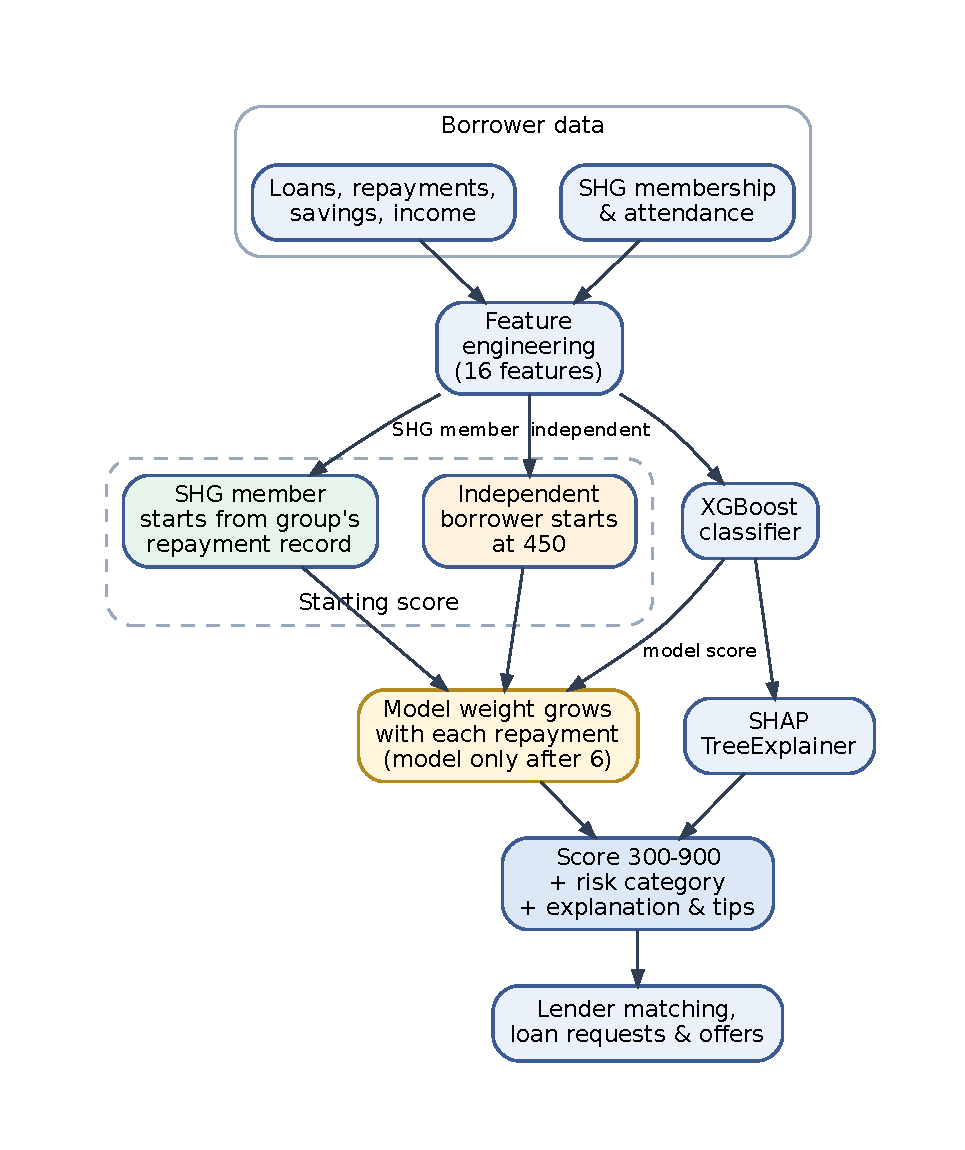
\includegraphics[width=0.62\textwidth]{fig/overview.pdf}
\caption{Overview of the dual-path scoring approach used in CreditSetu}
\label{fig:overview}
\end{figure}

An earlier version of this project (\texttt{Sahara MFI}, a Node/Express and
MySQL application) addressed SHG-only scoring through a hand-written SQL
formula, with no independent-borrower path, no machine-learning component
and no lender marketplace. CreditSetu is a from-scratch rebuild: the
general domain (SHGs, loans, repayments, credit scores) carries over, but
the schema, scoring approach and system design are new, driven by the
dual-path requirement that did not fit the old single-path schema.

\subsection{Problem Statement}
\begin{itemize}
  \item \textbf{Cold-start scoring:} an independent borrower with no formal
  credit history cannot be scored by a model trained only on borrowers who
  already have repayment history.
  \item \textbf{Opaque scoring:} even where a score exists, it is rarely
  explained in a way a borrower or a lender can act on.
  \item \textbf{No formal SHG--lender relationship:} lending decisions at
  group level are informal, unauditable and cannot be revoked cleanly.
  \item \textbf{Undifferentiated access:} in an open system a borrower, a
  lender and an SHG all see the same data, with no role-appropriate,
  access-controlled view for any of them.
\end{itemize}

\subsection{Objectives}
\begin{itemize}
  \item Build a dual-path scoring engine that gives SHG members a fair,
  group-earned head start while letting independent borrowers build a score
  purely from their own behaviour.
  \item Make every score explainable, feature by feature, using SHAP, and
  convert the negative contributions into improvement tips.
  \item Formalise the SHG--lender relationship as an explicit
  approve/reject linkage.
  \item Separate the system into four role-gated views (Borrower, Lender,
  SHG, Admin), each authorised server-side, so no role can see another's
  data.
  \item Let a borrower's own actions -- not just offline synthetic history
  -- move their own score, through a live repayment flow.
  \item Validate the system with an automated test suite covering
  functionality, access control and performance.
\end{itemize}

\subsection{Motivation}
Groups that repay reliably have already shown the kind of discipline a
lender cares about. The idea behind CreditSetu is to let that record give
each member a fair starting point, and then let each member's own
repayments take over. Borrowers without a group should still be able to
build a score from nothing, and both kinds of borrower should be told what
is affecting their score. The project was also chosen because it meets the
course selection criteria: it can be delivered in weekly increments, it is
locally relevant, and it can be built entirely with mature open-source
tools.

\subsection{Organisation of the Report}
Section~\ref{sec:related} reviews existing approaches.
Section~\ref{sec:req} gives the requirements analysis.
Section~\ref{sec:method} describes the proposed methodology: architecture,
data model, scoring, access control and the repayment flow.
Section~\ref{sec:feas} is the feasibility report.
Section~\ref{sec:impl} reports the implementation and the results measured
on the running system, and Section~\ref{sec:test} covers testing and
validation. Section~\ref{sec:concl} concludes. The use case diagram with
its written scenarios, the class diagram and the activity diagrams are
given in Appendices~\ref{sec:usecase-diagram}, \ref{sec:class-diagram} and
\ref{sec:activity-diagram}.

%==============================================================
\section{Related Work%
\BvrHint{\ldots existing approaches}}
\label{sec:related}

Traditional microfinance credit assessment relies heavily on group
liability and manual field-agent judgement, with limited use of statistical
or machine-learning scoring. Where formal credit bureaus exist (for example
CIBIL in India), they score individuals who already have a formal credit
history and have no mechanism for a first-time, group-affiliated borrower
to inherit a trust signal from their group. Commercial microfinance
information systems -- including the team's own earlier \texttt{Sahara MFI}
build -- typically implement a single, SHG-only scoring formula with no
cold-start path for independent borrowers and no per-feature explanation of
the resulting score.

Gradient-boosted decision trees, and XGBoost~\cite{xgboost} in particular,
are a standard choice for tabular credit-risk data: they cope with missing
values natively, need little feature scaling and train in seconds on
datasets of this size. Explainable-AI techniques such as SHAP~\cite{shap,
treeshap} have seen adoption in consumer credit scoring in developed
markets, where regulation increasingly demands a reason for an adverse
decision, but they are far less common in microfinance-specific tooling.
Isolation Forest~\cite{iforest} and $k$-means~\cite{kmeans} are established
methods for outlier detection and for grouping regions by behaviour, and
are used here for anomaly flags and district-level trust clustering
respectively.

What is missing in the existing work is the combination. Model opacity and
the cold-start problem are usually treated as separate, unrelated concerns.
CreditSetu addresses them together through an explicit bootstrap-to-model
blend whose weight is driven by how much of the borrower's own history has
accumulated, and through an explanation that covers the bootstrap
component as well as the model component.

%==============================================================
\section{Requirements Analysis%
\BvrHint{\ldots what the system must do}}
\label{sec:req}

\subsection{Stakeholders}
Table~\ref{tab:actors} lists the four user roles. Each role has its own
login and its own dashboard.

\begin{table}[H]
\centering
\caption{User roles and their main responsibilities}
\label{tab:actors}
\small
\begin{tabular}{@{}L{2.6cm}L{11.8cm}@{}}
\toprule
\textbf{Role} & \textbf{Responsibilities in CreditSetu}\\
\midrule
Borrower & View own score, history, explanation and tips; request loans; accept or reject offers; repay EMIs.\\
Self-Help Group & View group statistics and member scores; request or approve partnerships with lenders.\\
Lender & View reputation score; browse SHGs; manage partnerships; see eligible borrowers; make offers; approve or decline loan requests.\\
Admin (Bank) & Read-only oversight: portfolio summary, district clusters, anomaly flags, model health and borrower search.\\
\bottomrule
\end{tabular}
\end{table}

\subsection{Functional Requirements}
\begin{table}[H]
\centering
\caption{Functional requirements}
\label{tab:fr}
\small
\begin{tabular}{@{}lL{13.2cm}@{}}
\toprule
\textbf{ID} & \textbf{Requirement}\\
\midrule
FR1 & Provide separate logins for Borrower, Lender, SHG and Admin, and enforce role and ownership checks on the server (401 or 403).\\
FR2 & Compute a 300--900 score for every borrower from 16 engineered features, using the dual-path starting score when there is little or no history.\\
FR3 & Store every score as a new history row together with its SHAP explanation, and show up to five improvement tips.\\
FR4 & Let a borrower create, retarget and withdraw loan requests; a targeted request is visible only to its target lender.\\
FR5 & Let a lender approve (with an interest rate) or decline a request; approval creates an active loan, and a decline does not close the request for other lenders.\\
FR6 & Let a lender propose offers to eligible borrowers within its maximum loan amount; the borrower accepts or rejects.\\
FR7 & Manage SHG--lender partnerships; only the party that did not start the request may decide it.\\
FR8 & Calculate the EMI and total dues, block payment if the wallet cannot cover all dues, and record the repayment and the rescore in one transaction.\\
FR9 & Give the admin a portfolio summary, district clusters, anomaly detection, model health and borrower search.\\
\bottomrule
\end{tabular}
\end{table}

\subsection{Non-Functional Requirements}
\begin{table}[H]
\centering
\caption{Non-functional requirements and target values}
\label{tab:nfr}
\small
\begin{tabular}{@{}lL{3cm}L{10.2cm}@{}}
\toprule
\textbf{ID} & \textbf{Category} & \textbf{Requirement}\\
\midrule
NFR1 & Performance & Median response time of read endpoints below 300\,ms on the demonstration dataset.\\
NFR2 & Security & 100\% of cross-role or cross-identity requests refused; passwords stored only as salted hashes.\\
NFR3 & Accuracy & Scoring model holdout ROC-AUC at least 0.85 and accuracy at least 0.80.\\
NFR4 & Reliability & A payment and its rescore are atomic: a failed request leaves no partial change.\\
NFR5 & Scalability & Switch from SQLite to PostgreSQL through \code{DATABASE\_URL} only; all foreign keys indexed; list endpoints paginated.\\
NFR6 & Usability & Plain-language explanations; text-size, high-contrast and dark-mode controls.\\
NFR7 & Privacy & Only synthetic data; the public home page shows aggregate highlights only.\\
\bottomrule
\end{tabular}
\end{table}

\subsection{Use Case Model}
The system has 17 use cases across the four actors. They are shown as a use
case diagram in Appendix~\ref{sec:usecase-diagram},
Figure~\ref{fig:usecase}, together with written scenarios (pre-conditions,
main and alternate flows, exceptions and post-conditions) for the six most
important of them.

%==============================================================
\section{Proposed Methodology%
\BvrHint{\ldots system design}}
\label{sec:method}

\subsection{Technology Stack}
Table~\ref{tab:stack} lists the tools used to build the system. Every one
of them is mature, open-source and free of licensing cost.

\begin{table}[H]
\centering
\caption{Technology stack}
\label{tab:stack}
\small
\begin{tabular}{@{}L{3.4cm}L{11cm}@{}}
\toprule
\textbf{Layer} & \textbf{Technology}\\
\midrule
Frontend & React 19 single-page application, Vite, React Router, Recharts\\
Backend & Python 3.11, FastAPI (REST API with automatic OpenAPI docs), Uvicorn\\
Database & SQLAlchemy ORM over SQLite (demonstration); PostgreSQL through a configuration setting\\
Machine learning & XGBoost, SHAP, scikit-learn ($k$-means, Isolation Forest), pandas, NumPy\\
Data & Synthetic borrower population generated with Faker\\
Testing & pytest, FastAPI TestClient, Playwright (browser tests)\\
Tools & Git and GitHub, GitHub Actions (documentation site), PlantUML and Graphviz (diagrams)\\
\bottomrule
\end{tabular}
\end{table}

\subsection{System Architecture}
CreditSetu is a three-tier web application:
\begin{itemize}
  \item \textbf{Frontend:} a React (Vite) single-page application with four
  role-gated dashboards (Borrower, Lender, SHG, Admin) and a public landing
  page, styled as a government-portal-style demonstration platform (clearly
  labelled as such, and not impersonating any real government property).
  \item \textbf{Backend API:} FastAPI, exposing REST endpoints under
  \texttt{/api} through twelve routers, with bearer-token session
  authentication per role and server-side authorisation scoping every query
  to the authenticated caller's own identity. Routers delegate to service
  modules, which are the only place business rules live.
  \item \textbf{Database:} SQLAlchemy over SQLite for the demonstration
  deployment. A one-line \code{DATABASE\_URL} environment-variable change
  moves this to PostgreSQL for concurrent production use, with no code
  changes.
  \item \textbf{ML pipeline:} offline scripts (not imported by the API at
  request time) for synthetic data generation, model training and batch
  scoring, producing artifacts that the API loads once at start-up and then
  serves.
\end{itemize}

\subsection{Data Model}
The schema has 19 tables. The core of it is \texttt{districts},
\texttt{shgs} and \texttt{individuals}, where \texttt{individuals.shg\_id}
is the dual-path pivot: it is nullable, and NULL means the borrower is
independent. Around this sit \texttt{shg\_attendance\_records},
\texttt{savings\_records}, \texttt{lenders},
\texttt{shg\_lender\_links} (the approve/reject partnership table, carrying
an \texttt{initiated\_by\_role} column so the interface can tell which side
is entitled to decide a given link), \texttt{loans} (with a
borrower-chosen \texttt{target\_lender\_id} on the request side),
\texttt{repayment\_events}, \texttt{credit\_scores} (append-only score
history, not a single mutable column), \texttt{score\_explanations} (one
row per feature contribution, in score points, per score),
\texttt{loan\_offers} and \texttt{loan\_requests} (the two directions of
the marketplace), \texttt{anomaly\_flags}, and four separate
\texttt{\ldots\_sessions} tables, one per role. Every foreign key is
indexed, and unique constraints prevent duplicate partnerships and
duplicate declines. The full class-level detail of every table, field and
relationship is given in the class diagram in
Appendix~\ref{sec:class-diagram}.

\subsection{Scoring Approach}\label{sec:scoring}
Each borrower's score is computed in the following steps. The same process
is shown as an activity diagram in Appendix~\ref{sec:activity-diagram},
Figure~\ref{fig:activity}.
\begin{enumerate}
  \item \textbf{Collect data.} The system gathers the borrower's loans,
  repayments, savings, income and, for SHG members, meeting attendance, and
  turns them into 16 features such as the on-time repayment rate, the
  missed rate, the average days late and savings regularity. Missing data
  is marked as unknown rather than silently treated as zero.
  \item \textbf{Choose a starting score.} An SHG member starts from a score
  based mainly on how well the \emph{other} members of the group repay
  (weighted 60\% towards the group's own record and 40\% towards a neutral
  value of 500). An independent borrower starts from a flat 450.
  \item \textbf{Blend in the model.} If the borrower has no repayments yet,
  the starting score is used as it is and the model is not called. With
  each repayment event, more weight moves from the starting score to the
  XGBoost model's prediction. After six repayment events the model is used
  alone.
  \item \textbf{Explain the score.} SHAP contributions are converted into
  score points and saved as explanation rows, together with a row for the
  starting score while it still carries weight. Contributions are measured
  against the score of an average borrower rather than against the floor of
  300, so a borrower with a low score still receives a meaningful
  explanation instead of an almost empty one.
  \item \textbf{Assign a risk category and save.} The score is kept within
  300--900 and labelled Very Low risk (800 or more), Low (700--799), Medium
  (550--699), High (450--549) or Very High (below 450). Each run adds a new
  row to the borrower's score history, so older scores are never
  overwritten.
\end{enumerate}
Scoring runs for the whole population as a batch job, on demand when an
admin asks for a recompute, and automatically after every repayment.

\subsection{Role-Based Access Control}
Four roles -- Borrower, Lender, SHG and Admin -- log in separately (phone
and password for borrowers, username and password for the other three).
Passwords are stored only as salted PBKDF2-HMAC-SHA256
hashes~\cite{pbkdf2}. A successful login issues a random opaque session
token that expires after seven days; there is no JWT and no client-side
claim that the server trusts.

Every protected endpoint uses one of five FastAPI dependencies (one per
role, plus ``any logged-in role''). The borrower, lender or SHG that a
request refers to is always derived from the session and never taken from
the request body. An identifier appearing in a URL is checked against what
the session is entitled to see, and the server answers 401 when there is no
valid token and 403 when the caller is known but not entitled.
Table~\ref{tab:rbac} summarises what each role may see; this is enforced on
the server, not merely hidden in the interface.

\begin{table}[H]
\centering
\caption{Data access matrix (enforced on the server)}
\label{tab:rbac}
\small
\begin{tabular}{@{}L{3.6cm}L{2.5cm}L{3.3cm}L{2.4cm}L{2.4cm}@{}}
\toprule
\textbf{Data} & \textbf{Borrower} & \textbf{Lender} & \textbf{SHG} & \textbf{Admin}\\
\midrule
Own score, history, SHAP & Own only & -- & -- & All (read)\\
Other borrowers & Denied & Summary, linked SHGs or independents & Own members & All (read)\\
SHG details and members & Own SHG, no member list & Members if link is Approved & Own SHG & All (read)\\
Loan requests and offers & Own & Addressed to or made by them & Denied & All (read)\\
Partnership decisions & Denied & SHG-initiated links & Lender-initiated links & Denied\\
Anomalies, clusters, model health & Denied & Denied & Denied & Allowed\\
\bottomrule
\end{tabular}
\end{table}

\subsection{Loan Marketplace}
A lender is \emph{eligible} for a borrower if (i) the borrower is an SHG
member and that SHG has an Approved link with the lender, or the borrower
is independent and the lender serves independent borrowers, and (ii) the
borrower's latest score is at least the lender's minimum score. A borrower
may broadcast a loan request to every eligible lender or target one chosen
lender, and may retarget a pending request or withdraw it. A lender
approves a request with an interest rate, which creates an active loan, or
declines it; a decline only removes the request from that lender's queue
and leaves it pending for the others. In the other direction, a lender may
propose an offer to an eligible borrower within its maximum loan amount,
and the borrower accepts or rejects it.

To reward competitive pricing, in the spirit of the Reserve Bank of India's
priority-sector and co-lending incentives~\cite{rbi}, each lender carries a
reputation score from 0 to 100, where 50 is the platform average. The score
rises when the lender's base rate and the rates it actually offers are
below the platform average (the two heaviest factors), and rises further
with marketplace activity and with willingness to serve independent
borrowers. Borrowers see this score next to each suggested lender.

\subsection{Repayment and Payment Gateway}
Once a loan is active, the monthly instalment (EMI) is the principal plus
simple interest over the full tenure, divided equally across the months.
The amount due this cycle is derived from the count of existing repayment
events on that loan rather than from elapsed calendar time, so a loan is
payable as soon as it is disbursed instead of only after a real due date
has passed -- necessary for the feature to be usable by a live user rather
than only replayable against backdated data.

A demonstration payment gateway (clearly labelled as not real) shows the
borrower's wallet balance and the amount due per active loan. Before any
payment the server reloads the wallet and recomputes the borrower's
\emph{total} dues across all active loans; if the wallet cannot cover the
total, every payment is blocked, not just the one clicked, so a borrower
cannot clear one loan while silently defaulting on another. A successful
payment creates a real repayment event, reduces the outstanding balance,
closes the loan after the final instalment, debits the wallet and
recomputes the credit score -- all inside a single database transaction, so
a failure leaves no partial change. The full flow is shown as a swimlane
activity diagram in Appendix~\ref{sec:activity-diagram},
Figure~\ref{fig:swimlane}.

%==============================================================
\section{Feasibility Report%
\BvrHint{\ldots can this actually be built and run}}
\label{sec:feas}

\subsection{Technical Feasibility}
Every component uses mature, well-documented open-source tooling already
proven at this scale: FastAPI and SQLAlchemy for the API and the ORM,
XGBoost and SHAP for scoring and explanation, scikit-learn for $k$-means
district clustering and Isolation Forest anomaly detection, and
React/Vite for the frontend. No component requires novel research or
unavailable infrastructure. The dataset is small enough (1{,}079 borrowers,
494 training rows) that model training takes seconds on a two-core machine,
and the API serves the trained artifacts rather than retraining at request
time. The team has already built, run and fixed real defects in this stack
(Section~\ref{sec:bugs}), which demonstrates that the architecture is
technically sound in practice and not only on paper. The main technical
risk -- that the model would be unusable for borrowers without history --
is exactly what the dual-path starting score is designed to remove, and
that behaviour has been verified on the running system
(Section~\ref{sec:live}).

\subsection{Operational Feasibility}
The system runs on a single machine for demonstration (SQLite,
\code{uvicorn --reload}, \code{npm run dev}) with no dependency on any
external paid service. Each of the four stakeholder roles has a dashboard
built around the decision that role actually has to make, and the borrower
view deliberately avoids jargon: the score is accompanied by a
plain-language explanation and up to five concrete improvement tips, with
text-size, high-contrast and dark-mode controls for low-literacy and
low-vision users. A production deployment would swap SQLite for a managed
PostgreSQL instance through a single environment variable and replace the
deliberately minimal demonstration credential scheme with production-grade
hashing and short-lived signed tokens; both are additive changes, not
architectural rewrites. Field operation would additionally need an SHG
facilitator to keep attendance and savings records current, which is
already part of normal SHG practice.

\subsection{Economic Feasibility}
All tooling used is free and open-source, so there is no licensing cost.
Development cost is the team's own effort within the course timeline. At
production scale the only recurring cost would be standard cloud hosting --
a small managed database instance and an API/web server -- which is
proportionate to any comparable small-to-medium deployment and is not a
blocker for a course project or an early pilot. Because the scoring model
is trained offline and only the artifacts are loaded by the API, there is
no per-request inference cost and no paid model-serving dependency.

\subsection{Schedule Feasibility}
The eight-stage plan (synthetic data generation, scoring engine, cold-start
bootstrap, SHG--lender linkage, lender matching and offers, frontend,
geo-clustering, anomaly detection) was completed and verified end to end
before the current iteration began. The current iteration -- role
separation, server-side authorisation, targeted requests and the live
repayment flow -- is complete, tested against the live API and a real
browser, and documented with before/after verification
(Section~\ref{sec:impl}). Table~\ref{tab:sched} shows the remaining
milestones, which fit within the semester timeline because each is an
extension of working code rather than new construction.

\begin{table}[H]
\centering
\caption{Remaining schedule to the Final Report}
\label{tab:sched}
\small
\begin{tabular}{@{}L{3.2cm}L{7.4cm}L{3.6cm}@{}}
\toprule
\textbf{Milestone} & \textbf{Work} & \textbf{Status}\\
\midrule
Prototype stage, W7 (this report) & Role separation, live repayment flow, test suite, UML design & Complete\\
Hardening & Fix defects D-01 and D-02; production password and token scheme & Next\\
Analytics depth & Periodic re-scoring so score-history trends accumulate & Next\\
Admin actions & Moderation beyond the current read-only oversight, with an audit trail & Planned\\
Final Report & Fairness sensitivity analysis of the starting-score gap; full regression run & Planned\\
\bottomrule
\end{tabular}
\end{table}

%==============================================================
\section{Implementation and Results%
\BvrHint{\ldots what actually works, verified}}
\label{sec:impl}

All figures in this section are measured against the running system, not
estimated.

\subsection{Experimental Setup and Dataset}
The backend uses Python~3.11, FastAPI~0.115, SQLAlchemy~2.0, XGBoost~2.1,
SHAP~0.46 and scikit-learn~1.5; the frontend uses React~19 with Vite and
Recharts. All measurements were taken on a two-core Linux machine with
8\,GB of RAM. Because real borrower data is sensitive, the system uses a
reproducible synthetic population generated with Faker (random seed 42);
its size is given in Table~\ref{tab:data}. Defaults in the synthetic data
follow a smooth probabilistic rule based on missed, late and partial
payments rather than a hard threshold, which was itself the fix for an
early defect.

\begin{table}[H]
\centering
\caption{Seeded dataset}
\label{tab:data}
\small
\begin{tabular}{@{}lr@{\hskip 1.5cm}lr@{}}
\toprule
\textbf{Entity} & \textbf{Count} & \textbf{Entity} & \textbf{Count}\\
\midrule
Borrowers (total) & 1{,}079 & SHGs & 51\\
\quad SHG-linked & 659 & Lenders & 6\\
\quad Independent & 420 & Districts & 10\\
Loans & 1{,}619 & SHG--lender links & 97\\
\quad Defaulted & 315 (19.4\%) & Training rows for the model & 494\\
\bottomrule
\end{tabular}
\end{table}

\subsection{Scoring Model Performance}
The model is trained on SHG-linked borrowers with at least three repayment
events (494 rows), using an 80/20 stratified split. The hyperparameters are
200 trees, maximum depth 4, learning rate 0.05, and subsample and
column-sample ratios of 0.9. Table~\ref{tab:model} gives the holdout
results and the most important features.

\begin{table}[H]
\centering
\caption{Scoring model: holdout performance and top features by importance}
\label{tab:model}
\small
\begin{tabular}{@{}lr@{\hskip 1.5cm}lr@{}}
\toprule
\textbf{Metric} & \textbf{Value} & \textbf{Feature} & \textbf{Importance}\\
\midrule
Holdout accuracy & 0.909 & \code{missed\_rate} & 0.239\\
Holdout ROC-AUC & 0.962 & \code{on\_time\_rate} & 0.201\\
Training rows & 494 & \code{attendance\_rate} & 0.081\\
Test split & 20\% (stratified) & \code{n\_closed\_loans} & 0.048\\
Features & 16 & \code{avg\_days\_late} & 0.047\\
Borrowers scored & 1{,}079 / 1{,}079 & \code{n\_repayment\_events} & 0.045\\
\bottomrule
\end{tabular}
\end{table}

As expected, repayment behaviour (the missed and on-time rates) dominates,
followed by SHG meeting attendance. Both targets in NFR3 are met with a
wide margin. Figure~\ref{fig:dist} compares the latest scores of the two
borrower groups: SHG-linked borrowers average 718.7 against 675.0 for
independent borrowers. Many independent borrowers sit in the High-risk band
(450--549) precisely because their score starts at 450 and has not yet been
raised by repayments -- the dual-path design working as intended rather
than a defect.

\begin{figure}[H]
\centering
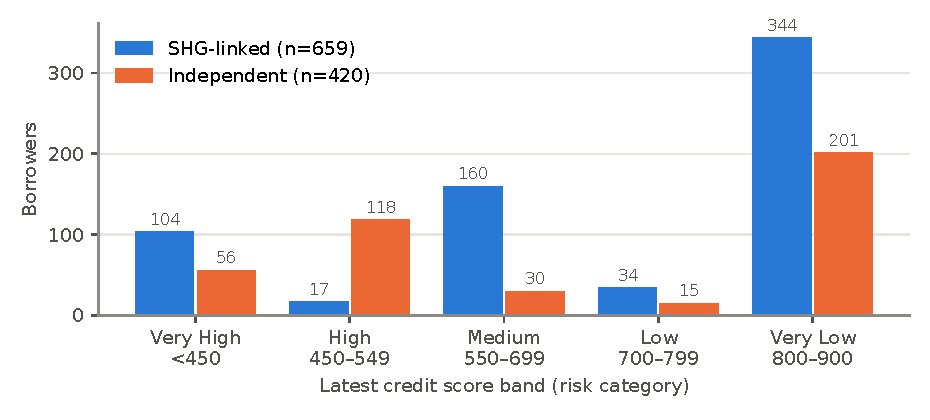
\includegraphics[width=0.9\textwidth]{fig/chart_scores.pdf}
\caption{Distribution of latest credit scores by risk band for SHG-linked and independent borrowers}
\label{fig:dist}
\end{figure}

\subsection{Live Validation and Performance}\label{sec:live}
A seeded SHG member was taken through the full flow on the live system with
no manual database edits. The borrower requested Rs.~15{,}000 for 12 months
from District Cooperative Bank, the lender approved it at 12.5\% (an EMI of
Rs.~1{,}406.25), and the borrower paid four instalments on time. The score
rose from 717 to 898 and the scoring basis switched from the blended
starting score to the model alone once the borrower reached six repayment
events (Figure~\ref{fig:live}a) -- exactly the behaviour specified in
Section~\ref{sec:scoring}.

Median response times measured on the running server are shown in
Figure~\ref{fig:live}b. Login is deliberately slow (about 120\,ms, because
of PBKDF2 with 200{,}000 iterations); every read endpoint is far below the
300\,ms target of NFR1, the slowest being the eligible-borrowers list at
about 154\,ms.

\begin{figure}[H]
\centering
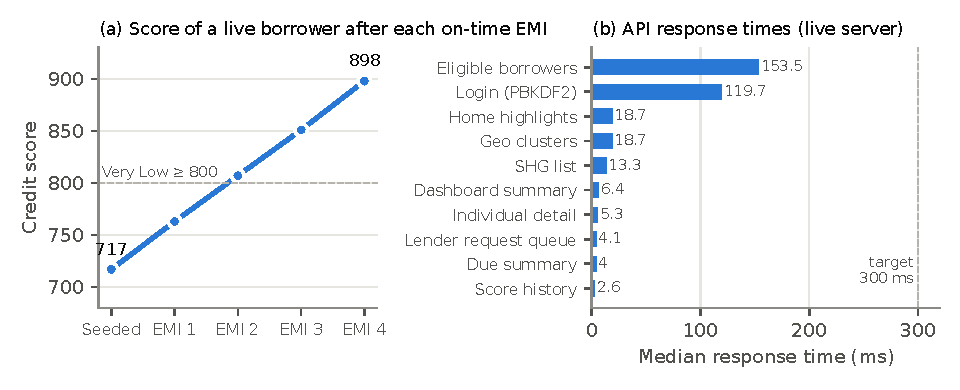
\includegraphics[width=\textwidth]{fig/chart_results.pdf}
\caption{(a) Score of a live borrower after each on-time EMI; (b) median API response times}
\label{fig:live}
\end{figure}

\subsection{User Interface}
Figures~\ref{fig:ui1} and~\ref{fig:ui2} show screens captured from the
running application.

\begin{figure}[H]
\centering
\begin{subfigure}[t]{0.49\textwidth}\centering
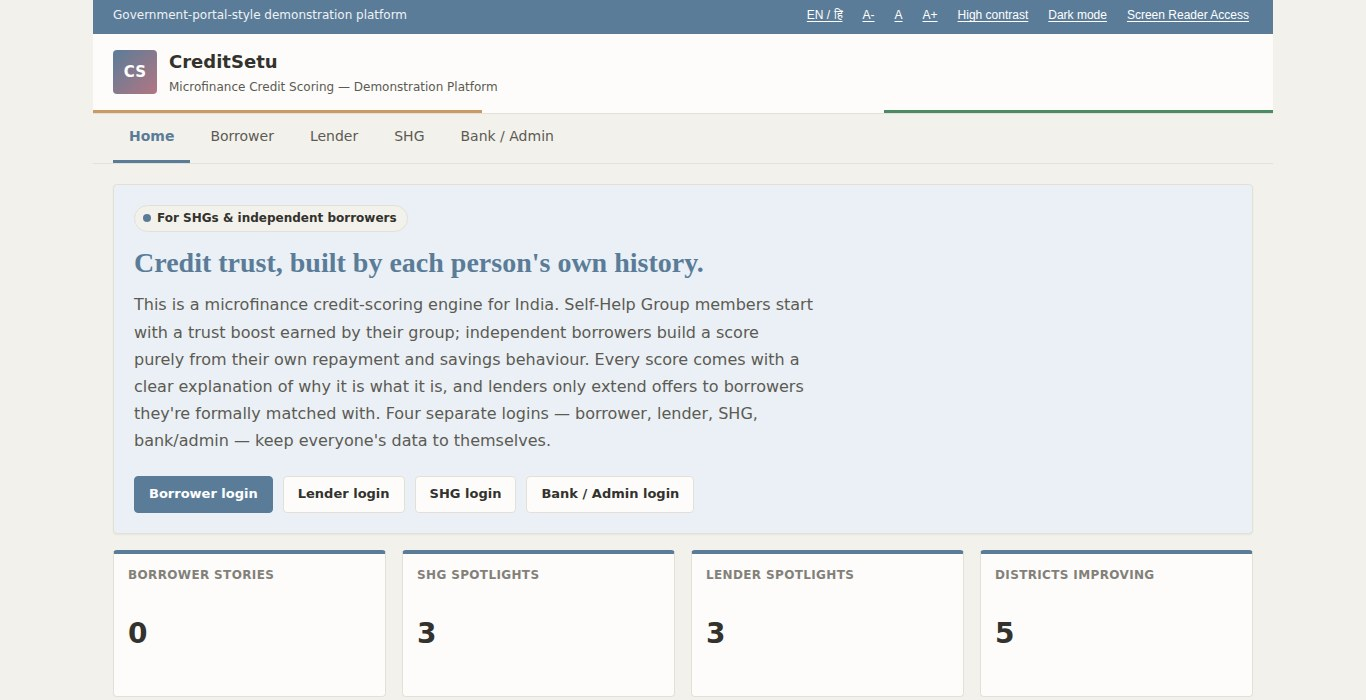
\includegraphics[width=\textwidth]{shots/ss_home_hero.jpg}
\caption{Public home page with role logins}
\end{subfigure}\hfill
\begin{subfigure}[t]{0.49\textwidth}\centering
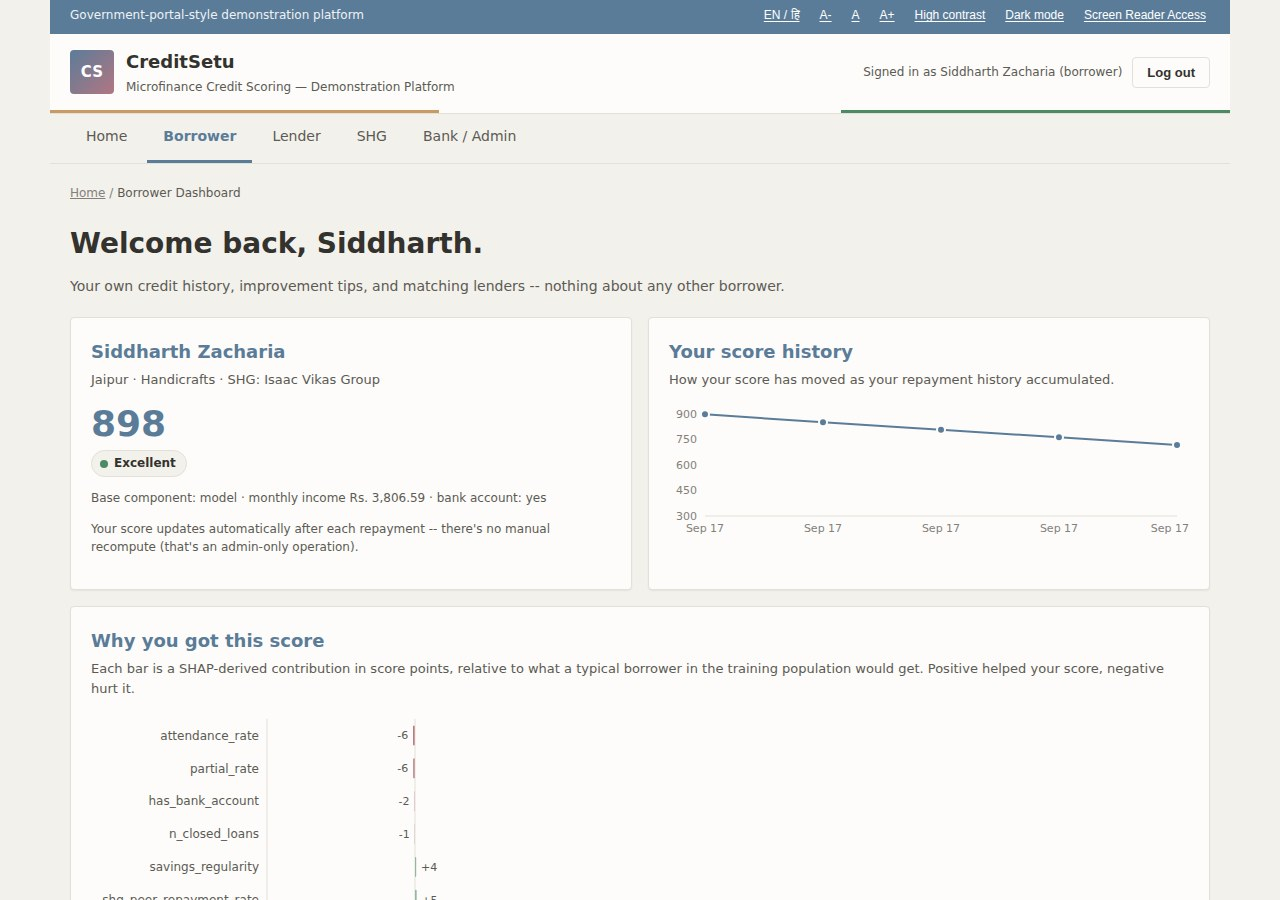
\includegraphics[width=\textwidth]{shots/ss_b_top.jpg}
\caption{Borrower dashboard and score history}
\end{subfigure}\\[6pt]
\begin{subfigure}[t]{0.49\textwidth}\centering
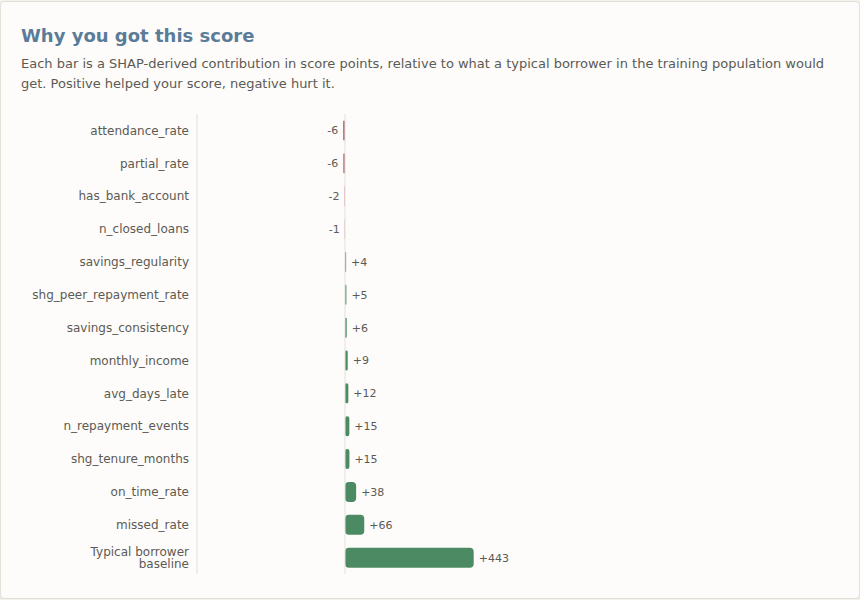
\includegraphics[width=\textwidth]{shots/b_shap.png}
\caption{``Why you got this score'' (SHAP)}
\end{subfigure}\hfill
\begin{subfigure}[t]{0.49\textwidth}\centering
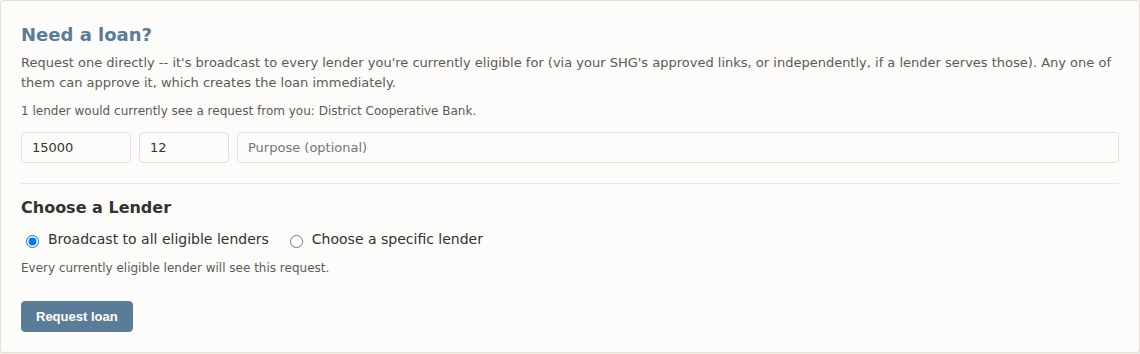
\includegraphics[width=\textwidth]{shots/ss_b_need.jpg}
\caption{Loan request (broadcast or targeted)}
\end{subfigure}\\[6pt]
\begin{subfigure}[t]{0.24\textwidth}\centering
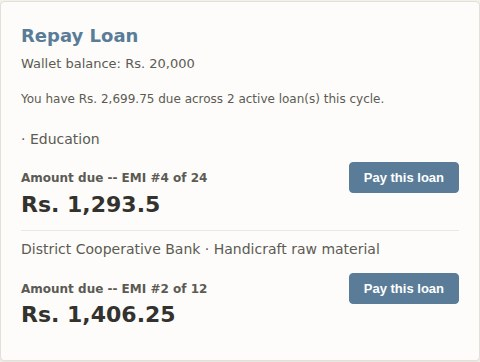
\includegraphics[width=\textwidth]{shots/ss_pay_before.jpg}
\caption{Repay page}
\end{subfigure}\hfill
\begin{subfigure}[t]{0.24\textwidth}\centering
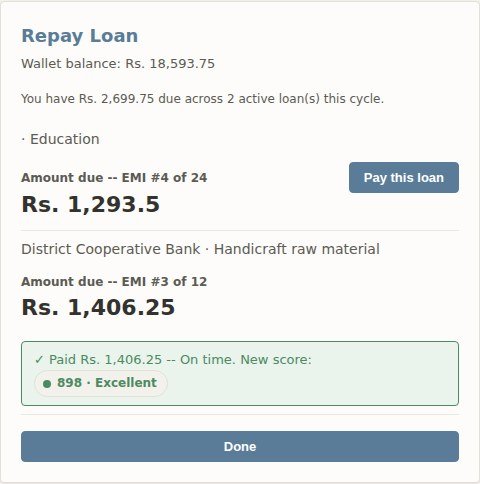
\includegraphics[width=\textwidth]{shots/ss_pay_after.jpg}
\caption{After payment}
\end{subfigure}\hfill
\begin{subfigure}[t]{0.49\textwidth}\centering
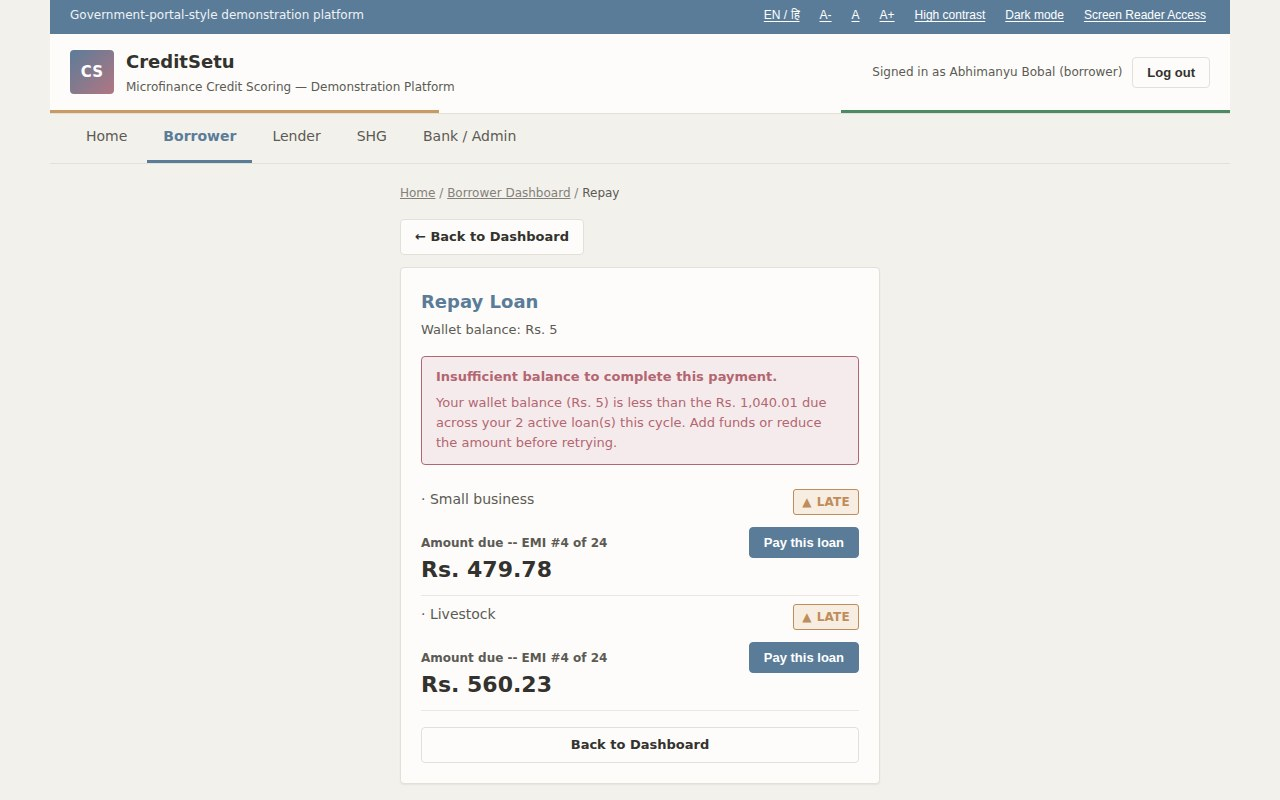
\includegraphics[width=\textwidth]{shots/ss_pay_blocked.jpg}
\caption{Payment blocked: insufficient wallet}
\end{subfigure}
\caption{Borrower screens}
\label{fig:ui1}
\end{figure}

\begin{figure}[H]
\centering
\begin{subfigure}[t]{0.49\textwidth}\centering
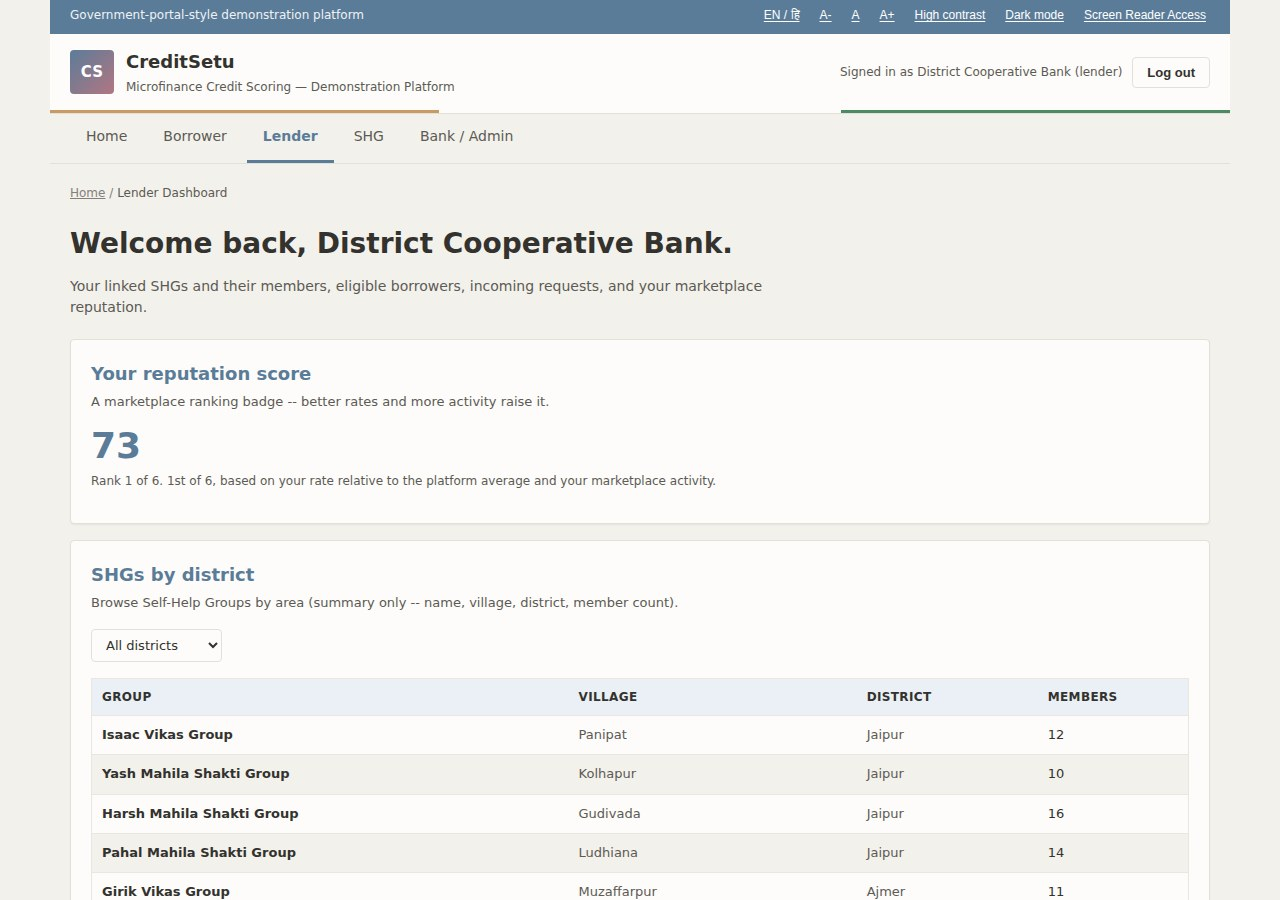
\includegraphics[width=\textwidth]{shots/ss_l_top.jpg}
\caption{Lender dashboard with reputation}
\end{subfigure}\hfill
\begin{subfigure}[t]{0.49\textwidth}\centering
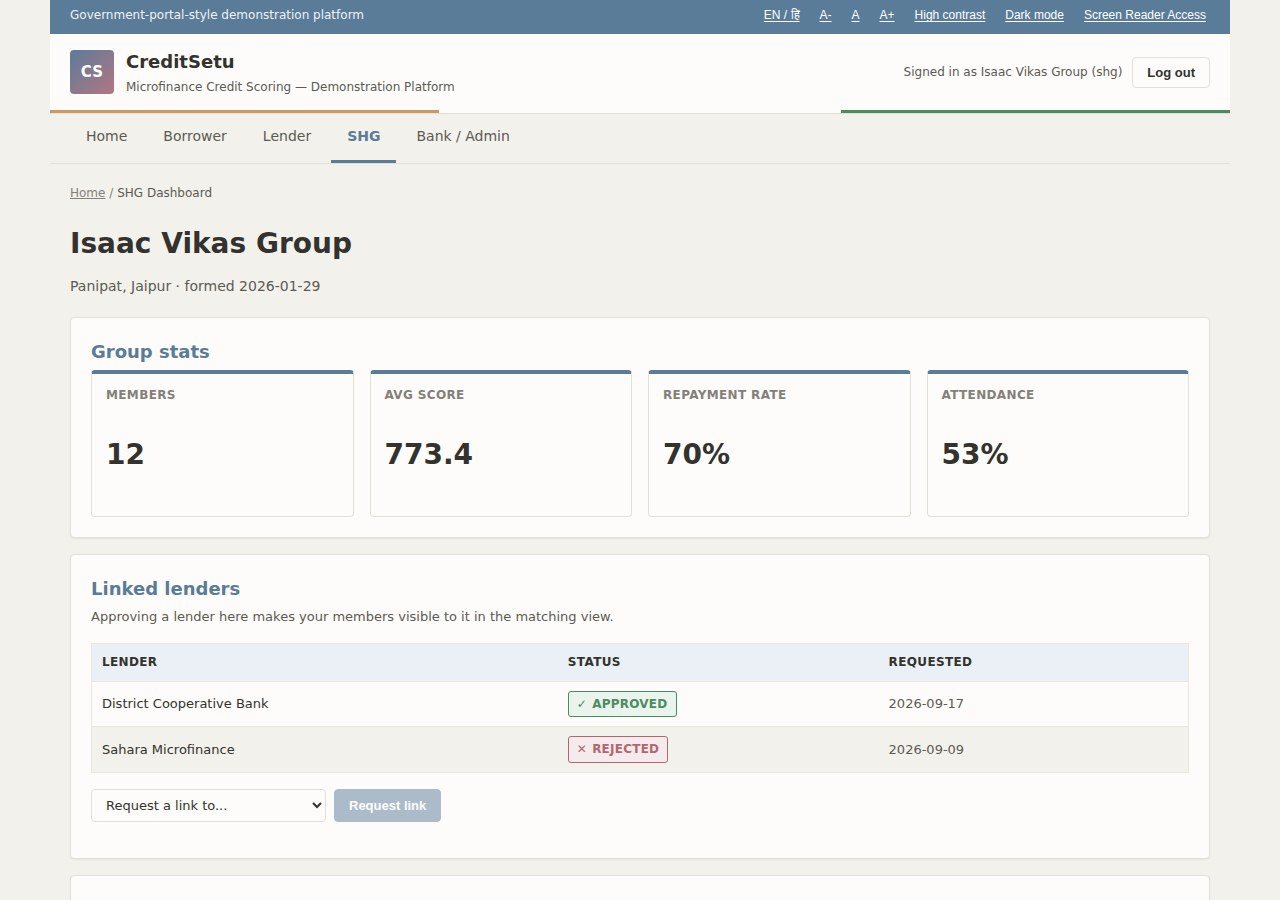
\includegraphics[width=\textwidth]{shots/ss_s_top.jpg}
\caption{SHG dashboard}
\end{subfigure}\\[6pt]
\begin{subfigure}[t]{0.49\textwidth}\centering
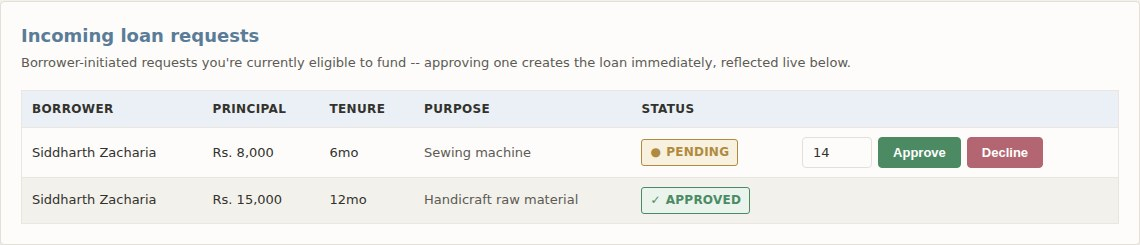
\includegraphics[width=\textwidth]{shots/ss_l_in.jpg}
\caption{Lender: incoming loan requests}
\end{subfigure}\hfill
\begin{subfigure}[t]{0.49\textwidth}\centering
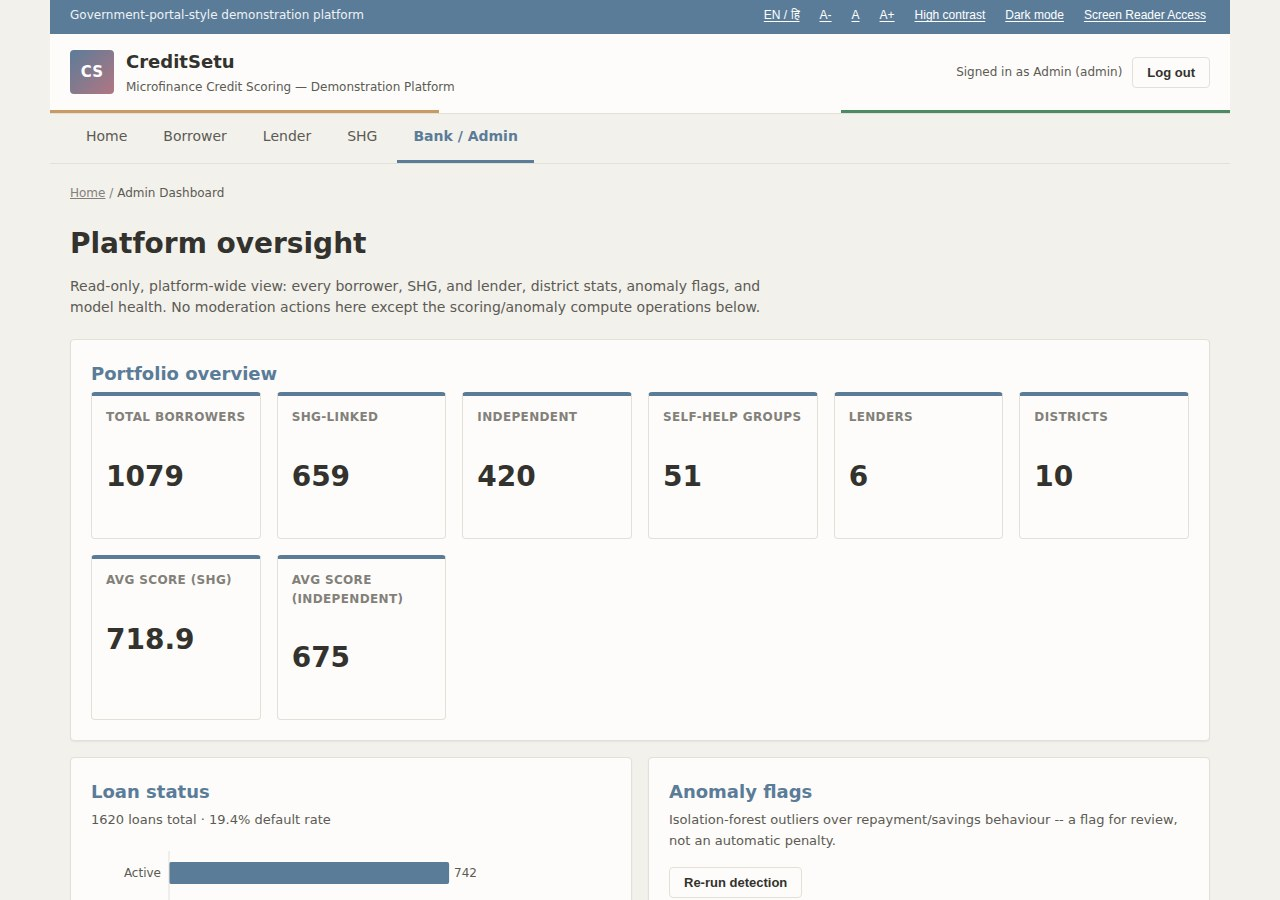
\includegraphics[width=\textwidth]{shots/ss_a_top.jpg}
\caption{Admin: platform overview}
\end{subfigure}\\[6pt]
\begin{subfigure}[t]{0.49\textwidth}\centering
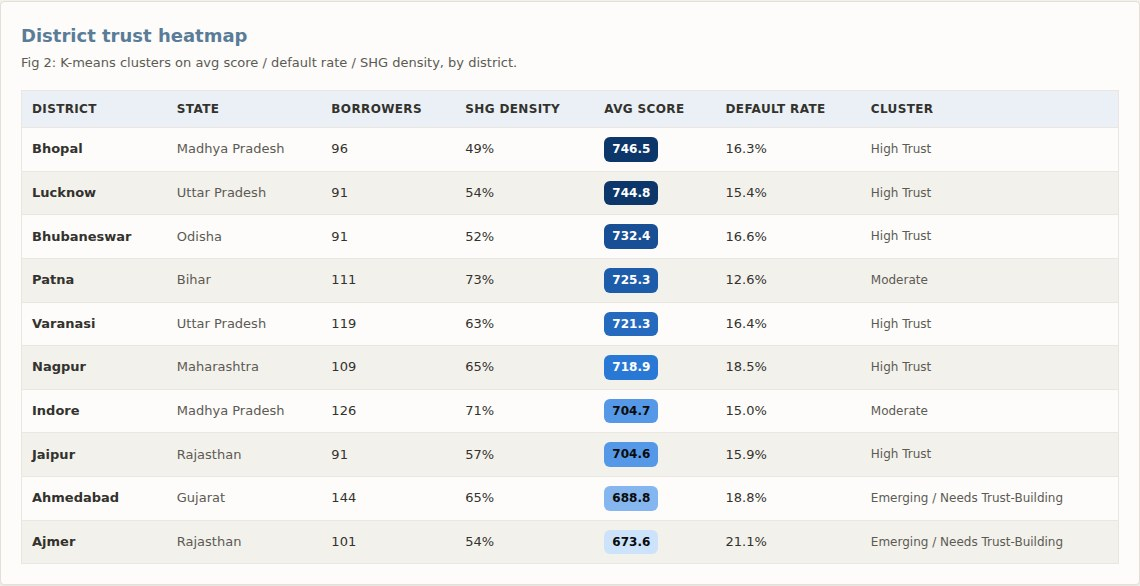
\includegraphics[width=\textwidth]{shots/ss_a_heat.jpg}
\caption{Admin: district trust heatmap ($k$-means)}
\end{subfigure}\hfill
\begin{subfigure}[t]{0.49\textwidth}\centering
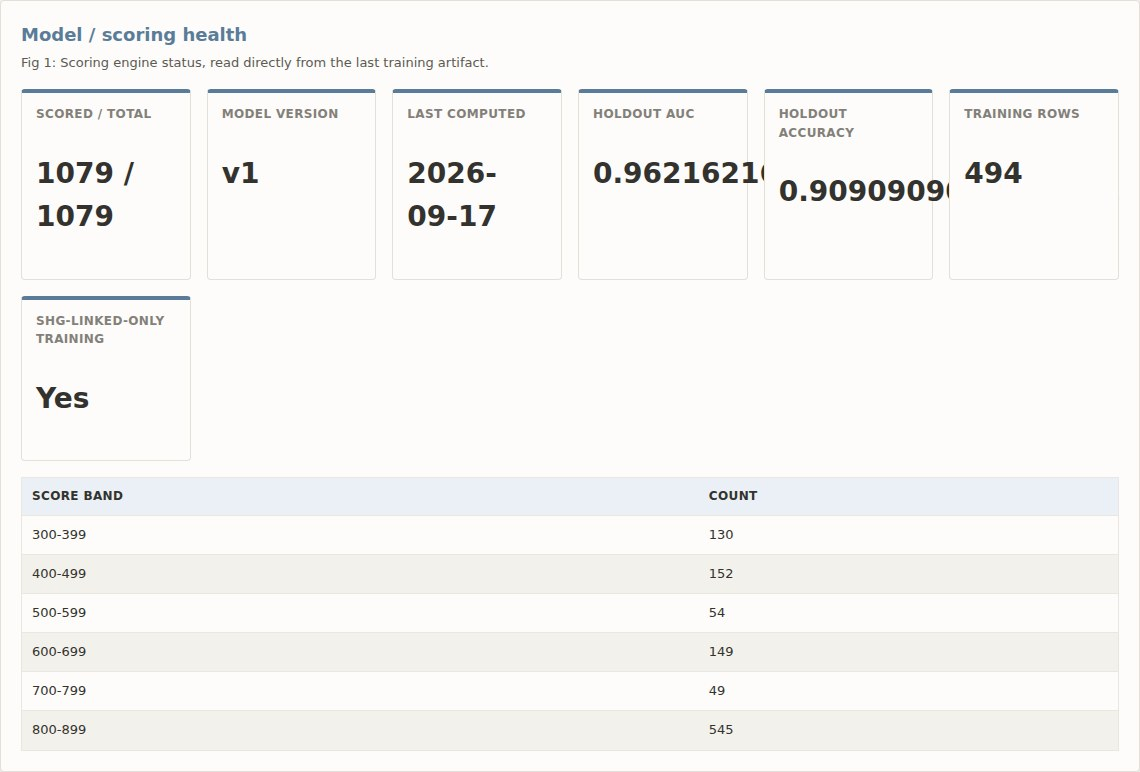
\includegraphics[width=\textwidth]{shots/ss_a_model.jpg}
\caption{Admin: model health}
\end{subfigure}
\caption{Lender, SHG and Admin screens}
\label{fig:ui2}
\end{figure}

\subsection{Defects Found and Fixed During Development}
\label{sec:bugs}
Running the system end to end -- training on the real dataset, calling the
live API and exercising the live frontend -- rather than only reading the
code revealed several defects that shaped the design
(Table~\ref{tab:bugs}). Two of them were silent: nothing crashed and
nothing looked empty, which is precisely why they survived code review.

\begin{table}[H]
\centering
\caption{Main defects found and fixed during development}
\label{tab:bugs}
\small
\begin{tabular}{@{}L{7.2cm}L{7.2cm}@{}}
\toprule
\textbf{Defect} & \textbf{Fix}\\
\midrule
A hard \code{missed\_fraction > 0.4} cliff made the synthetic default label a near coin-flip at the boundary & Replaced with a smooth, probabilistic default rule\\
SHAP explanation was almost empty for high-risk borrowers, who need it most & Share points above the population baseline instead of above the floor of 300\\
$k$-means cluster labels were inverted, so the worst districts were labelled ``High Trust'' & Label clusters by the rank of their mean score\\
Approve/Reject Partnership buttons sent an undefined field (\code{link\_id} instead of \code{id}), so a lender could never actually decide a link & Corrected the field name and verified the flow live\\
Search could reach only about half of the borrowers (interface limit of 1000 against an API cap of 500) & Search moved to the server (\code{?search=}) with a debounced input\\
\code{GET /api/shgs} used an N+1 query walking members, loans and repayment events per SHG (1.1--1.3\,s) & Three \code{GROUP BY} aggregates: about 13\,ms, a 75$\times$ improvement with identical content\\
Foreign keys were not indexed, and the eligible-borrower table rendered 351 rows uncapped & Indexes added; table capped at 25 rows with a ``top N of M'' note\\
\bottomrule
\end{tabular}
\end{table}

%==============================================================
\section{Testing and Validation%
\BvrHint{\ldots does it do what it claims}}
\label{sec:test}

\subsection{Test Strategy}
The goal of testing is to confirm that each role can do exactly what it is
allowed to do and nothing more, that scores are correct at the boundaries,
and that money-related actions are atomic. Test cases were designed with
equivalence partitioning (valid, invalid and unauthorised inputs) and
boundary value analysis (risk bands and the ends of the score range), then
automated at the three levels shown in Table~\ref{tab:levels}. API tests
run against a temporary copy of the seeded database, so the demonstration
data is never modified, and the borrower/lender pairs used by a test are
chosen at run time from the current eligibility rules instead of being
hard-coded, so the suite does not silently rot as the data changes.

\begin{table}[H]
\centering
\caption{Test levels and tools}
\label{tab:levels}
\small
\begin{tabular}{@{}L{2.6cm}L{6.6cm}L{3.1cm}L{2cm}@{}}
\toprule
\textbf{Level} & \textbf{What is tested} & \textbf{Tool} & \textbf{Cases}\\
\midrule
Unit & Scoring formulas, risk boundaries, reputation logic & pytest & 8\\
Integration (API) & REST endpoints with real tokens: authentication, access control, marketplace, payments, links, offers, analytics & pytest + FastAPI TestClient & 38\\
System (end-to-end) & User journeys in a real browser & Playwright (Chromium) & 8\\
\midrule
\multicolumn{3}{@{}l}{\textbf{Total}} & \textbf{54}\\
\bottomrule
\end{tabular}
\end{table}

\subsection{Test Cases and Results}
Table~\ref{tab:tcd} gives the step-by-step form of one representative test
case, and Table~\ref{tab:tc} lists all 54 test cases with their expected
and actual results from the run of 17 September 2026. Parameterised cases
(TC04 over 3 roles and TC21 over 9 boundary scores) run several times, so
there are 64 executions in total; the whole suite completes in 28\,s.

\begin{table}[H]
\centering
\caption{Detailed test case: EMI repayment through the payment gateway}
\label{tab:tcd}
\small
\begin{tabular}{@{}lL{4.0cm}L{4.2cm}L{3.1cm}l@{}}
\toprule
\multicolumn{5}{@{}l}{\textbf{Test case:} TC32--TC35, E2E05--06 \quad \textbf{Subsystem:} Payments \quad \textbf{Executed:} 17/09/2026}\\
\multicolumn{5}{@{}l}{\textbf{Pre-condition:} borrower has an active loan of Rs.~6{,}000 at 12\% for 6 months (EMI = Rs.~1{,}060)}\\
\midrule
\textbf{Step} & \textbf{Action} & \textbf{Expected} & \textbf{Actual} & \textbf{Status}\\
\midrule
1 & Open due summary & Total = sum of EMIs; sufficient if wallet $\ge$ total & Consistent & \pass\\
2 & Pay with wallet Rs.~1{,}00{,}000 & Rs.~1{,}060 paid, On\_Time, balance 4{,}940, wallet 98{,}940, new score & As expected & \pass\\
3 & Pay with wallet Rs.~1 & 400 \code{insufficient\_funds}, no change & Outstanding still 6{,}000 & \pass\\
4 & Another borrower pays this loan & 403 & 403 & \pass\\
5 & UI: click \emph{Pay this loan} & ``New score'' shown & ``898 $\cdot$ Excellent'' & \pass\\
6 & UI: wallet of Rs.~5 & Every payment blocked, shortfall shown & Banner shown & \pass\\
\midrule
\multicolumn{5}{@{}l}{\textbf{Post-condition:} repayment, balance, wallet and score change together, or not at all.}\\
\bottomrule
\end{tabular}
\end{table}

\small
\begin{longtable}{@{}lL{1.95cm}L{4.3cm}L{2.9cm}L{2.5cm}l@{}}
\caption{Test cases and results}\label{tab:tc}\\
\toprule
\textbf{ID} & \textbf{Module} & \textbf{Test case} & \textbf{Expected} & \textbf{Actual} & \textbf{Status}\\
\midrule
\endfirsthead
\toprule
\textbf{ID} & \textbf{Module} & \textbf{Test case} & \textbf{Expected} & \textbf{Actual} & \textbf{Status}\\
\midrule
\endhead
\bottomrule
\endfoot
TC01 & Auth & Borrower login with valid phone and password & 200 + token & 200, token issued & \pass\\
TC02 & Auth & Borrower login with wrong password & 401 ``Incorrect\dots'' & 401 & \pass\\
TC03 & Auth & Login with an unregistered phone number & 401 & 401 & \pass\\
TC04 & Auth & Lender, SHG and admin login (3 runs) & 200 each & 200 each & \pass\\
TC05 & Auth & Admin login with wrong password & 401 & 401 & \pass\\
TC06 & Auth & Protected endpoints called without a token & 401 & 401 & \pass\\
TC07 & Auth & Reuse a token after logout & 401 & 401 & \pass\\
TC08 & Auth & Each account has a uniquely salted hash & Different hashes & All 1{,}079 borrowers share one hash & \fail\\
TC09 & RBAC & Borrower reads another borrower's record & 403 & 403 & \pass\\
TC10 & RBAC & Borrower calls admin-only borrower list & 403 & 401 (still denied) & \fail\\
TC11 & RBAC & Admin lists the population & 200 & 200 & \pass\\
TC12 & RBAC & Lender opens an unlinked SHG & 403 & 403 & \pass\\
TC13 & RBAC & Lender opens an approved-linked SHG & 200 with members & 200 with members & \pass\\
TC14 & RBAC & Borrower opens own SHG & Summary, no members & As expected & \pass\\
TC15 & RBAC & Anomaly flags for borrower vs admin & Denied / 200 & Denied / 200 & \pass\\
TC16 & RBAC & Public home highlights without login & 200 & 200 & \pass\\
TC17 & Scoring & New independent borrower (0 repayments) & Exactly 450 & 450 & \pass\\
TC18 & Scoring & New SHG member (0 repayments) & Group-based start, above 450 & As expected & \pass\\
TC19 & Scoring & All stored scores within range & 300--900 & In range & \pass\\
TC20 & Scoring & Explanation rows add up to score $-$ 300 & Within tolerance & Within tolerance & \pass\\
TC21 & Scoring & Risk band at 9 boundary scores & Correct band & 9/9 correct & \pass\\
TC22 & Scoring & Probability-to-score conversion & Scores 300, 600, 900 at the ends and middle & As expected & \pass\\
TC23 & Scoring & Model quality targets & AUC $\ge$0.85, acc. $\ge$0.80 & 0.962 / 0.909 & \pass\\
TC24 & Requests & Principal = 0 & 400 & 400 & \pass\\
TC25 & Requests & Target an ineligible lender & 400 & 400 & \pass\\
TC26 & Requests & Targeted request visibility & Only target lender & Only target lender & \pass\\
TC27 & Requests & Lender declines a broadcast request & Still Pending & Pending, hidden from that lender & \pass\\
TC28 & Requests & Approve without an interest rate & 400 & 400 & \pass\\
TC29 & Requests & Approve with rate 12\% & Active loan created & Loan Active, balance 6{,}000 & \pass\\
TC30 & Requests & Withdraw the same request twice & Withdrawn, then 400 & As expected & \pass\\
TC31 & Requests & Withdraw another borrower's request & 403 & 403 & \pass\\
TC32 & Payments & Due-summary totals & Sum of EMIs & Consistent & \pass\\
TC33 & Payments & Pay EMI (Rs.~6{,}000, 12\%, 6 months) & Rs.~1{,}060 paid, On\_Time, new score & Exactly as expected & \pass\\
TC34 & Payments & Wallet of Rs.~1 & 400, nothing changed & 400, balance unchanged & \pass\\
TC35 & Payments & Pay another borrower's loan & 403 & 403 & \pass\\
TC36 & Links & SHG requests; SHG self-approves; lender approves & Pending; 403; Approved & As expected & \pass\\
TC37 & Links & Duplicate partnership request & 400 & 400 & \pass\\
TC38 & Links & Re-decide an approved link & 400 & 400 & \pass\\
TC39 & Links & Admin tries to decide a link & 403 & 403 & \pass\\
TC40 & Offers & Offer to an ineligible borrower & 400 & 400 & \pass\\
TC41 & Offers & Offer above the maximum loan amount & 400 & 400 & \pass\\
TC42 & Offers & Wrong borrower, then right borrower, accepts & 403; loan created & As expected & \pass\\
TC43 & Analytics & Lower base rate increases reputation & Higher score & Higher score & \pass\\
TC44 & Analytics & Best district is labelled High Trust & Correct label & Correct & \pass\\
TC45 & Analytics & Dashboard counts add up & Consistent & Consistent & \pass\\
TC46 & Performance & Median time of \code{GET /api/shgs} & $<300$\,ms & $\approx$13\,ms & \pass\\
E2E01 & UI & Borrower login opens own dashboard & Welcome + SHAP card & Shown & \pass\\
E2E02 & UI & Wrong password message & ``Incorrect credentials.'' & Shown & \pass\\
E2E03 & UI & Open /admin without a session & Redirect to login & Redirected & \pass\\
E2E04 & UI & Borrower session opens /lender & Lender data not shown & Not shown & \pass\\
E2E05 & UI & Pay an EMI from the Repay page & ``New score'' shown & Shown & \pass\\
E2E06 & UI & Repay with a wallet of Rs.~5 & Blocked banner & Shown & \pass\\
E2E07 & UI & Lender dashboard content & Reputation + requests & Shown & \pass\\
E2E08 & UI & Log out, then open /shg & Redirect to login & Redirected & \pass\\
\end{longtable}
\normalsize

\subsection{Test Summary}
Table~\ref{tab:summary} summarises the results by module: 52 of 54 test
cases passed (96.3\%).

\begin{table}[H]
\centering
\caption{Test summary by module}
\label{tab:summary}
\small
\begin{tabular}{@{}lccccL{4.6cm}@{}}
\toprule
\textbf{Module} & \textbf{Cases} & \textbf{Passed} & \textbf{Failed} & \textbf{Pass rate} & \textbf{Observation}\\
\midrule
Authentication & 11 & 10 & 1 & 90.9\% & Shared seeded hash (D-01)\\
Access control & 10 & 9 & 1 & 90\% & 401 instead of 403 (D-02); no data leaked\\
Scoring engine & 7 & 7 & 0 & 100\% & Starting scores exact; AUC 0.962\\
Loan requests & 8 & 8 & 0 & 100\% & Rules enforced on the server\\
Payments & 6 & 6 & 0 & 100\% & Atomic; blocked on low funds\\
Partnerships and offers & 7 & 7 & 0 & 100\% & Only the correct party can decide\\
Analytics and performance & 5 & 5 & 0 & 100\% & Median $\approx$13\,ms\\
\midrule
\textbf{Total} & \textbf{54} & \textbf{52} & \textbf{2} & \textbf{96.3\%} & \\
\bottomrule
\end{tabular}
\end{table}

\subsection{Defect Report}
\begin{table}[H]
\centering
\caption{Open defects found by testing}
\label{tab:defects}
\small
\begin{tabular}{@{}lL{5.9cm}L{1.9cm}L{4.9cm}@{}}
\toprule
\textbf{ID} & \textbf{Description} & \textbf{Severity} & \textbf{Recommended fix}\\
\midrule
D-01 & \code{data\_gen.py} hashes the demonstration password once and reuses the result, so all 1{,}079 seeded borrowers share one salt and hash. Lender and SHG hashes are unique. & Low (demo data) & Call \code{hash\_password()} separately for each borrower.\\
D-02 & Admin-only endpoints answer 401 ``Not logged in'' to a valid borrower, lender or SHG token instead of 403 as the specification requires. Access is still denied. & Low & Return 403 in \code{get\_current\_admin} when the token belongs to another role's valid session.\\
\bottomrule
\end{tabular}
\end{table}

Both defects are low severity and neither exposes any data: D-01 concerns
seeded demonstration accounts only, and D-02 refuses the request correctly
but with the wrong status code, which misleads the frontend rather than the
security check. Every other functional requirement and every measurable
target (NFR1--NFR4) was met.

%==============================================================
\section{Conclusion and Future Scope%
\BvrHint{\ldots where this stands and what's next}}
\label{sec:concl}

At the prototype stage CreditSetu has a working, explainable, dual-path
scoring engine; a formal SHG--lender linkage; a two-directional loan
marketplace with targeted requests; four separately authorised role-based
views with server-side access control; and a live borrower repayment flow
whose effect on the credit score has been verified on a real account rather
than merely claimed, with a score rising from 717 to 898 across four
on-time instalments. The XGBoost model reaches a holdout ROC-AUC of 0.962
and an accuracy of 0.909, every score is explained with SHAP and turned
into improvement tips, and 52 of 54 automated test cases pass. Real
defects, including one that silently broke a core lender action and one
with a measured 75$\times$ performance impact, were found and fixed by
exercising the live system rather than only reading the code.

Remaining work towards the Final Report: fixing defects D-01 and D-02;
replacing the deliberately minimal demonstration credential scheme with a
vetted password-hashing library and short-lived signed tokens; periodic
re-scoring so that genuine score-history trends accumulate over time
(currently limited by how few times the batch-scoring pipeline has been
run); admin moderation actions beyond the present read-only oversight, with
an audit trail; integration with a real payment provider and EMI reminders;
retraining on real data with a time-based train/test split; and a mobile,
multilingual interface for rural borrowers. The gap between the independent
and SHG starting scores remains a stated policy parameter rather than
something derived from the data, and is flagged as a candidate for a
fairness sensitivity analysis in the Final Report.

\section*{Data and Code Availability}
The source code, documentation and synthetic data generator are available
at \url{https://github.com/shreesh1802/ucs503p-202627-Microfinance-Project}.



%==============================================================
\newpage
\appendix
\section{Use Case Diagram}
\label{sec:usecase-diagram}

Figure~\ref{fig:usecase} shows the four actors (Borrower, Self-Help Group,
Lender and Admin) against every use case, each of which is grounded in an
API router and a dashboard that exist in the code. Log In / Log Out and the
lender directory are shared by several actors; the remaining use cases
belong to a single role. Two \emph{include} relationships are worth noting:
viewing the score always includes generating the improvement tips from it,
and repaying an EMI always includes recomputing the credit score, which is
why a repayment cannot leave the score stale.

\vspace*{\fill}
\begin{figure}[H]
\centering
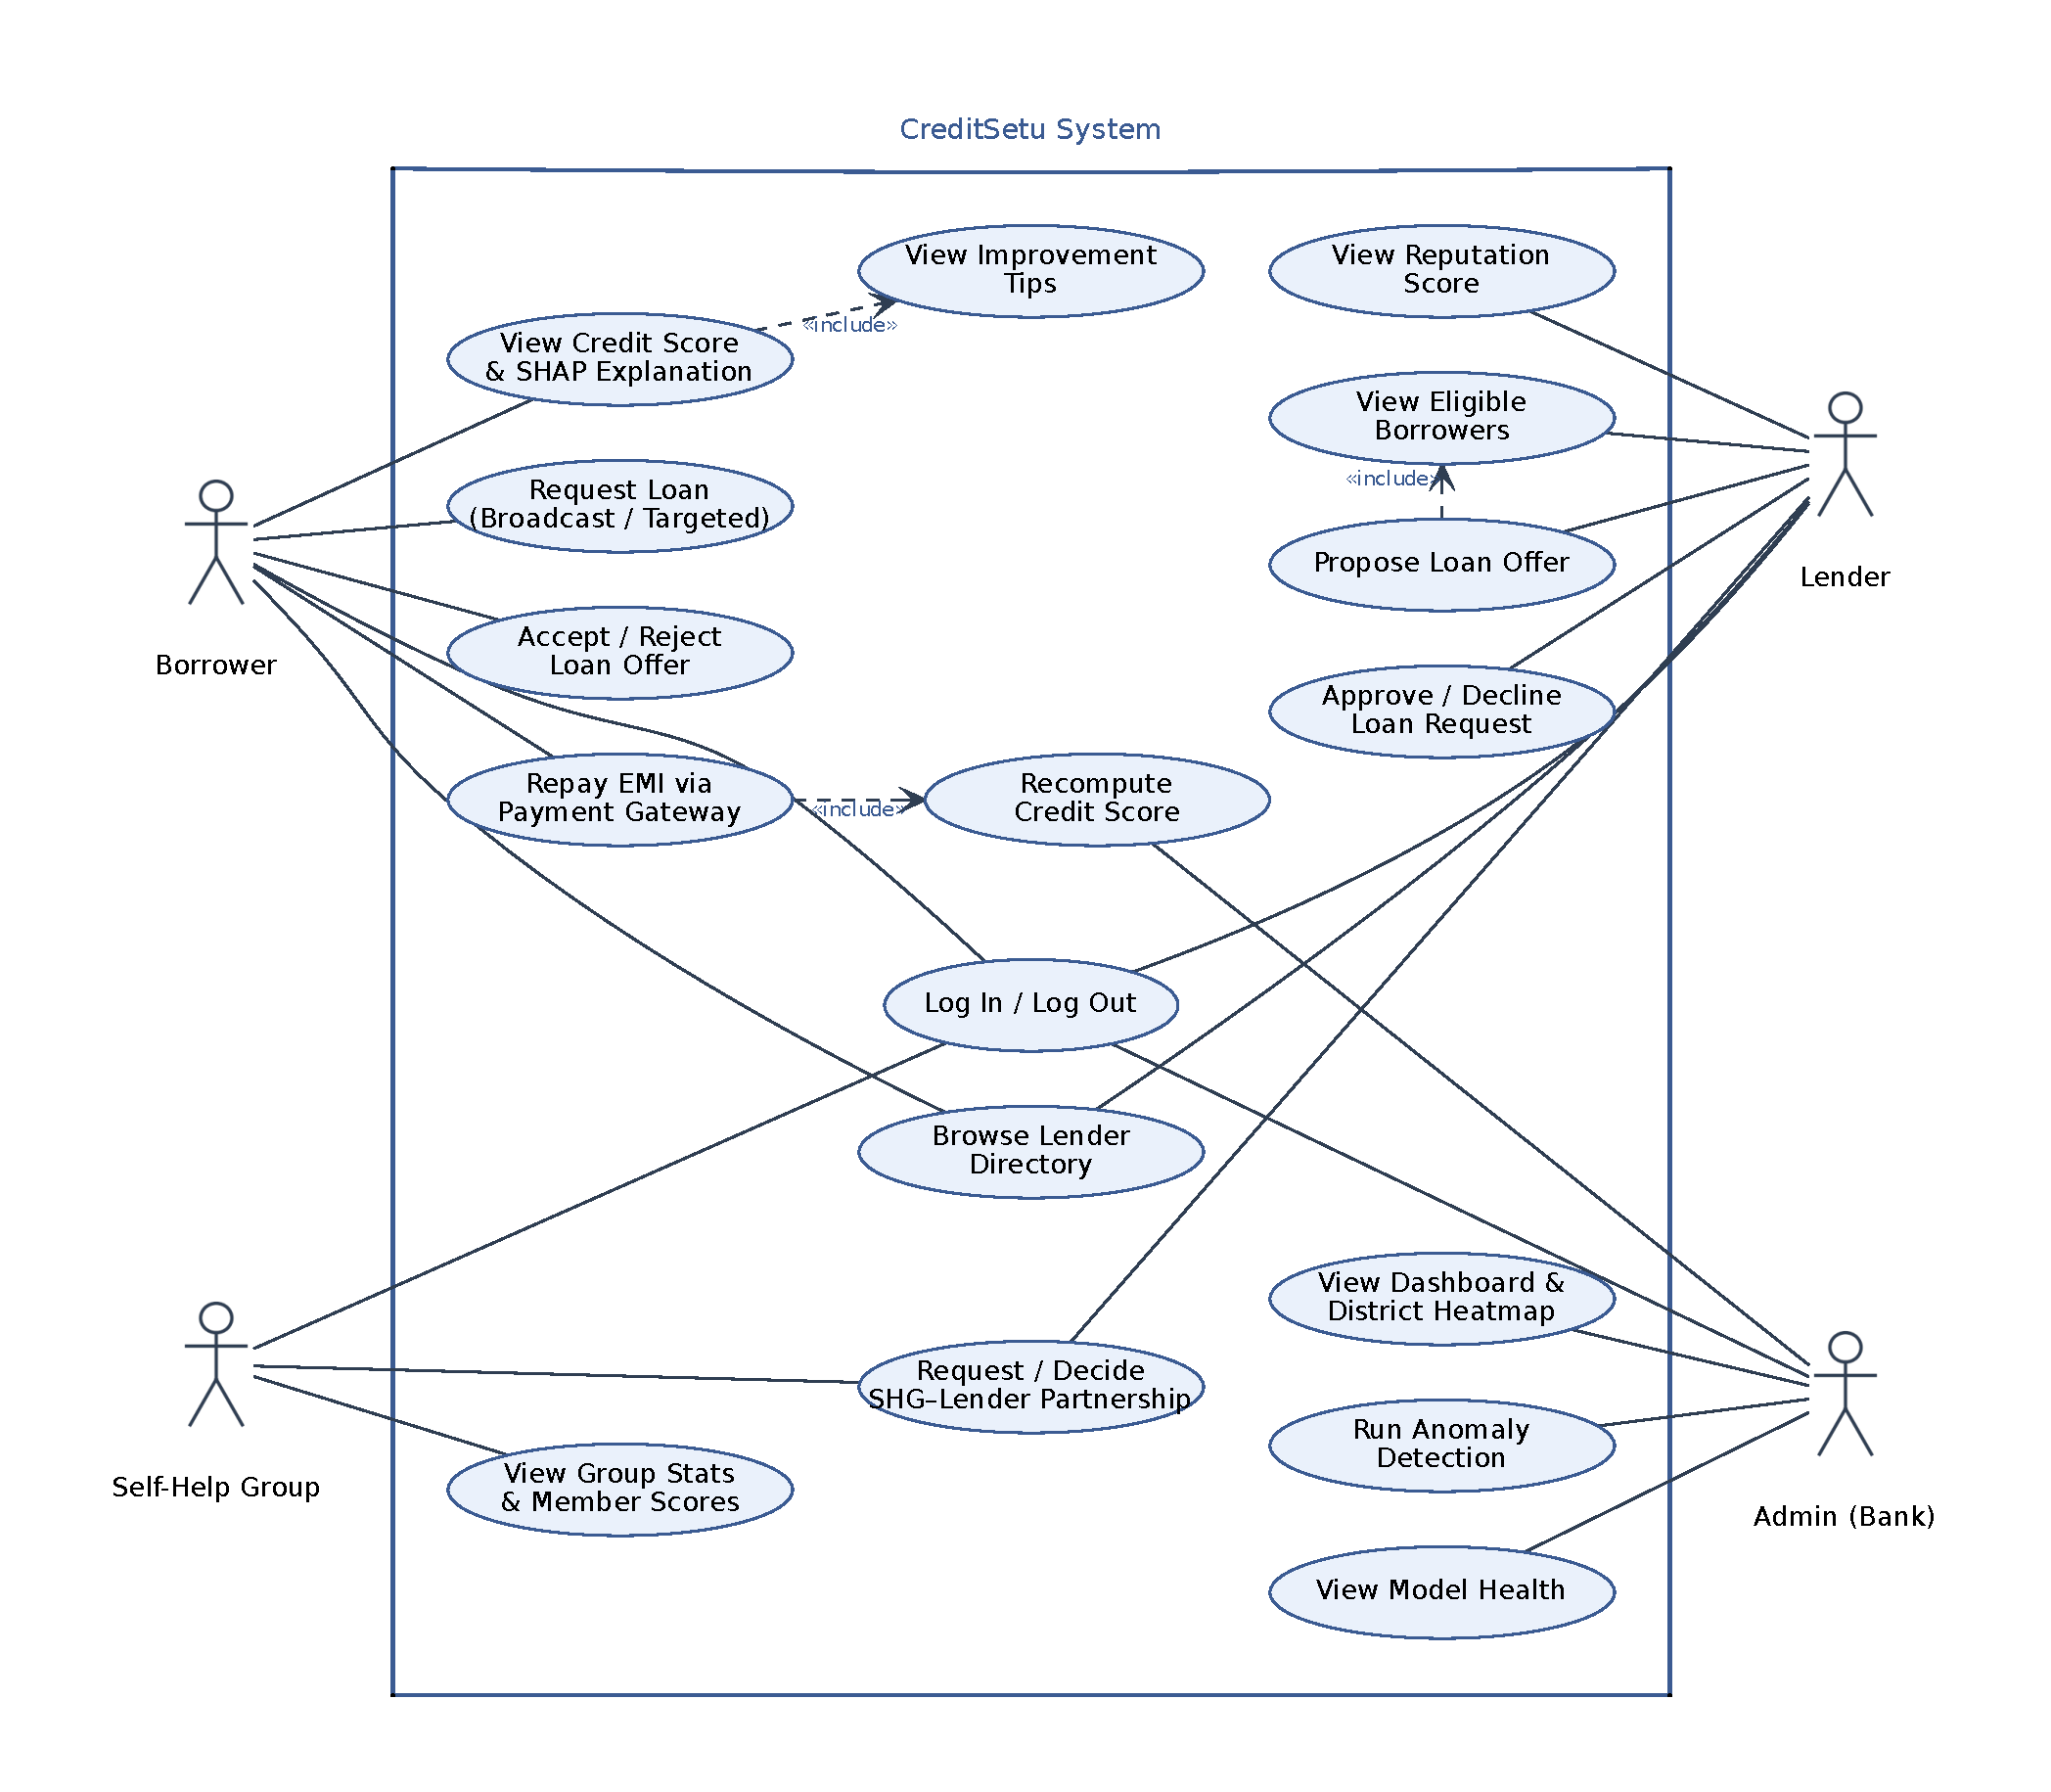
\includegraphics[width=\textwidth]{fig/use_case.pdf}
\caption{Use case diagram of CreditSetu}
\label{fig:usecase}
\end{figure}
\vspace*{\fill}

\clearpage
\subsection*{Use Case Scenarios}
\addcontentsline{toc}{subsection}{Use Case Scenarios}
Tables~\ref{tab:uc1}--\ref{tab:uc6} give the written scenarios for the six
most important use cases. HTTP status codes in the exception rows are the
codes the API actually returns.

\begin{table}[H]
\centering
\caption{Use case specification: Log In}
\label{tab:uc1}
\small
\begin{tabular}{@{}L{3.1cm}L{11.3cm}@{}}
\toprule
\textbf{Use case} & UC01: Log In (role-gated)\\
\textbf{Actors} & Borrower, Self-Help Group, Lender, Admin\\
\textbf{Pre-conditions} & The account exists in the seeded demonstration data; the user has opened the login page for their role.\\
\textbf{Main flow} & (1) User selects a role and submits credentials: phone and password for a borrower, username and password for the other three roles. (2) System looks up the account for that role only. (3) System verifies the password against the stored salted PBKDF2 hash. (4) System creates a row in that role's session table and returns an opaque bearer token valid for seven days. (5) The frontend stores the token and opens that role's dashboard.\\
\textbf{Alternate flows} & The user logs out, which deletes the session row; any later call with the same token is refused.\\
\textbf{Exceptions} & Unknown identifier or wrong password: HTTP 401 with the message ``Incorrect credentials.'' and no indication of which of the two was wrong. A token used against another role's endpoints is refused.\\
\textbf{Post-conditions} & A session row exists for exactly one role, and the caller's identity for every later request is taken from that session rather than from the request body.\\
\bottomrule
\end{tabular}
\end{table}

\begin{table}[H]
\centering
\caption{Use case specification: View Credit Score and Explanation}
\label{tab:uc2}
\small
\begin{tabular}{@{}L{3.1cm}L{11.3cm}@{}}
\toprule
\textbf{Use case} & UC02: View Credit Score, Explanation and Improvement Tips\\
\textbf{Actor} & Borrower (Admin may read any borrower's score)\\
\textbf{Pre-conditions} & Borrower is logged in and has at least one stored score.\\
\textbf{Main flow} & (1) System takes the borrower's id from the session. (2) System returns the latest score, its risk band and the scoring basis (starting score, blended or model). (3) System returns the score history so the dashboard can draw the trend. (4) System returns the stored per-feature contributions in score points. (5) The dashboard shows them as a bar chart and converts the negative contributions into up to five plain-language improvement tips.\\
\textbf{Alternate flows} & An admin may trigger a recompute, which appends a new score row rather than overwriting the existing one.\\
\textbf{Exceptions} & Requesting another borrower's score: HTTP 403. No token: HTTP 401.\\
\textbf{Post-conditions} & Nothing is modified; the score history is read-only from this use case.\\
\bottomrule
\end{tabular}
\end{table}

\begin{table}[H]
\centering
\caption{Use case specification: Request a Loan}
\label{tab:uc3}
\small
\begin{tabular}{@{}L{3.1cm}L{11.3cm}@{}}
\toprule
\textbf{Use case} & UC03: Request a Loan (broadcast or targeted)\\
\textbf{Actor} & Borrower\\
\textbf{Pre-conditions} & Borrower is logged in and has a credit score.\\
\textbf{Main flow} & (1) Borrower enters principal, tenure and an optional purpose. (2) Borrower chooses \emph{broadcast} or one specific eligible lender. (3) System takes the borrower's id from the session and checks that the principal and tenure are positive. (4) For a targeted request, system checks that the lender is still eligible: an approved SHG link or willingness to serve independents, and a score at or above the lender's minimum. (5) System saves the request as \emph{Pending} and shows it under ``Your loan requests''.\\
\textbf{Alternate flows} & Borrower retargets a pending request to another lender or back to broadcast, or withdraws it.\\
\textbf{Exceptions} & Invalid amount or ineligible target: HTTP 400 with a message. Acting on another borrower's request: HTTP 403. Withdrawing an already withdrawn request: HTTP 400.\\
\textbf{Post-conditions} & The request appears in the queue of every eligible lender, or only in the target lender's queue.\\
\bottomrule
\end{tabular}
\end{table}

\begin{table}[H]
\centering
\caption{Use case specification: Approve or Decline a Loan Request}
\label{tab:uc4}
\small
\begin{tabular}{@{}L{3.1cm}L{11.3cm}@{}}
\toprule
\textbf{Use case} & UC04: Approve or Decline a Loan Request\\
\textbf{Actor} & Lender\\
\textbf{Pre-conditions} & Lender is logged in; at least one pending request is addressed to it, either directly or by broadcast.\\
\textbf{Main flow} & (1) Lender opens the incoming request queue, which contains only requests it is eligible for. (2) Lender opens a request and sees the borrower's score, risk band and path (SHG-linked or independent). (3) To approve, the lender enters an interest rate. (4) System re-checks eligibility and the lender's maximum loan amount at the moment of the decision, not at the moment of the request. (5) System marks the request approved and creates an Active loan with its outstanding balance and EMI schedule.\\
\textbf{Alternate flows} & The lender declines: the request is hidden from that lender but remains \emph{Pending} for every other eligible lender, and the same lender cannot decline it twice.\\
\textbf{Exceptions} & Approval without an interest rate: HTTP 400. Deciding a request addressed to another lender, or an admin attempting to decide: HTTP 403. Re-deciding a request that is no longer pending: HTTP 400.\\
\textbf{Post-conditions} & Either an Active loan exists and the request is closed, or the request remains open for other lenders. No intermediate state is stored.\\
\bottomrule
\end{tabular}
\end{table}

\begin{table}[H]
\centering
\caption{Use case specification: Repay EMI through the Payment Gateway}
\label{tab:uc5}
\small
\begin{tabular}{@{}L{3.1cm}L{11.3cm}@{}}
\toprule
\textbf{Use case} & UC05: Repay EMI\\
\textbf{Actor} & Borrower\\
\textbf{Pre-conditions} & Borrower is logged in, has at least one active loan and has signed in to the demonstration gateway.\\
\textbf{Main flow} & (1) System shows the wallet balance, the EMI for each active loan and the total due this cycle. (2) Borrower clicks \emph{Pay this loan}. (3) System reloads the wallet and recalculates the total due on the server, ignoring the values the page was showing. (4) System records the repayment as \emph{On\_Time} or \emph{Late}, debits the EMI from the wallet, reduces the outstanding balance and closes the loan after the final instalment. (5) System recomputes the credit score and commits everything in one transaction. (6) The page shows the new score.\\
\textbf{Alternate flows} & A late payment is recorded with the number of days late, which feeds the \code{avg\_days\_late} feature at the next scoring run.\\
\textbf{Exceptions} & Wallet below the \emph{total} dues across all active loans: HTTP 400 \code{insufficient\_funds}, and every payment is blocked, not only the one clicked. Paying another borrower's loan: HTTP 403.\\
\textbf{Post-conditions} & Loan, wallet and score history are updated together, or not at all.\\
\bottomrule
\end{tabular}
\end{table}

\begin{table}[H]
\centering
\caption{Use case specification: Request and Decide an SHG--Lender Partnership}
\label{tab:uc6}
\small
\begin{tabular}{@{}L{3.1cm}L{11.3cm}@{}}
\toprule
\textbf{Use case} & UC06: Request / Decide an SHG--Lender Partnership\\
\textbf{Actors} & Self-Help Group, Lender\\
\textbf{Pre-conditions} & Both parties exist; no approved or pending link already joins them.\\
\textbf{Main flow} & (1) Either party browses the other (an SHG browses the lender directory, a lender browses SHGs by district) and sends a partnership request. (2) System stores the link as \emph{Pending} together with the role that initiated it. (3) The other party sees it in its pending list and approves or rejects it. (4) On approval the link becomes \emph{Approved}, and from that moment the lender may see that SHG's member list and its members may target that lender.\\
\textbf{Alternate flows} & Either party may later revoke an approved partnership, after which member visibility is withdrawn.\\
\textbf{Exceptions} & The initiating side deciding its own request: HTTP 403 (only the other party may decide). A duplicate request, or a decision on an already-decided link: HTTP 400. An admin attempting to decide: HTTP 403, because that decision belongs to the two named parties.\\
\textbf{Post-conditions} & Exactly one link row exists for the pair, in state Pending, Approved or Rejected, with a record of which side initiated it.\\
\bottomrule
\end{tabular}
\end{table}

\clearpage
\section{Class Diagram}
\label{sec:class-diagram}

Figure~\ref{fig:class} shows the domain model, which matches the
SQLAlchemy schema in \code{app/models.py}. Three design decisions are
visible in it:

\begin{itemize}
  \item \code{Individual.shg\_id} is optional, and a missing value marks an
  independent borrower. This single nullable association carries the whole
  dual-path design without duplicating tables or splitting the population
  into two parallel schemas.
  \item \code{CreditScore} is append-only and carries its own
  \code{ScoreExplanation} rows, so any past score and the reason for it can
  be reconstructed later. Nothing overwrites a score in place.
  \item \code{SHGLenderLink} is a many-to-many association table that also
  records its own state and which side initiated it, which is what makes
  the approve/reject rule enforceable.
\end{itemize}

\begin{figure}[H]
\centering
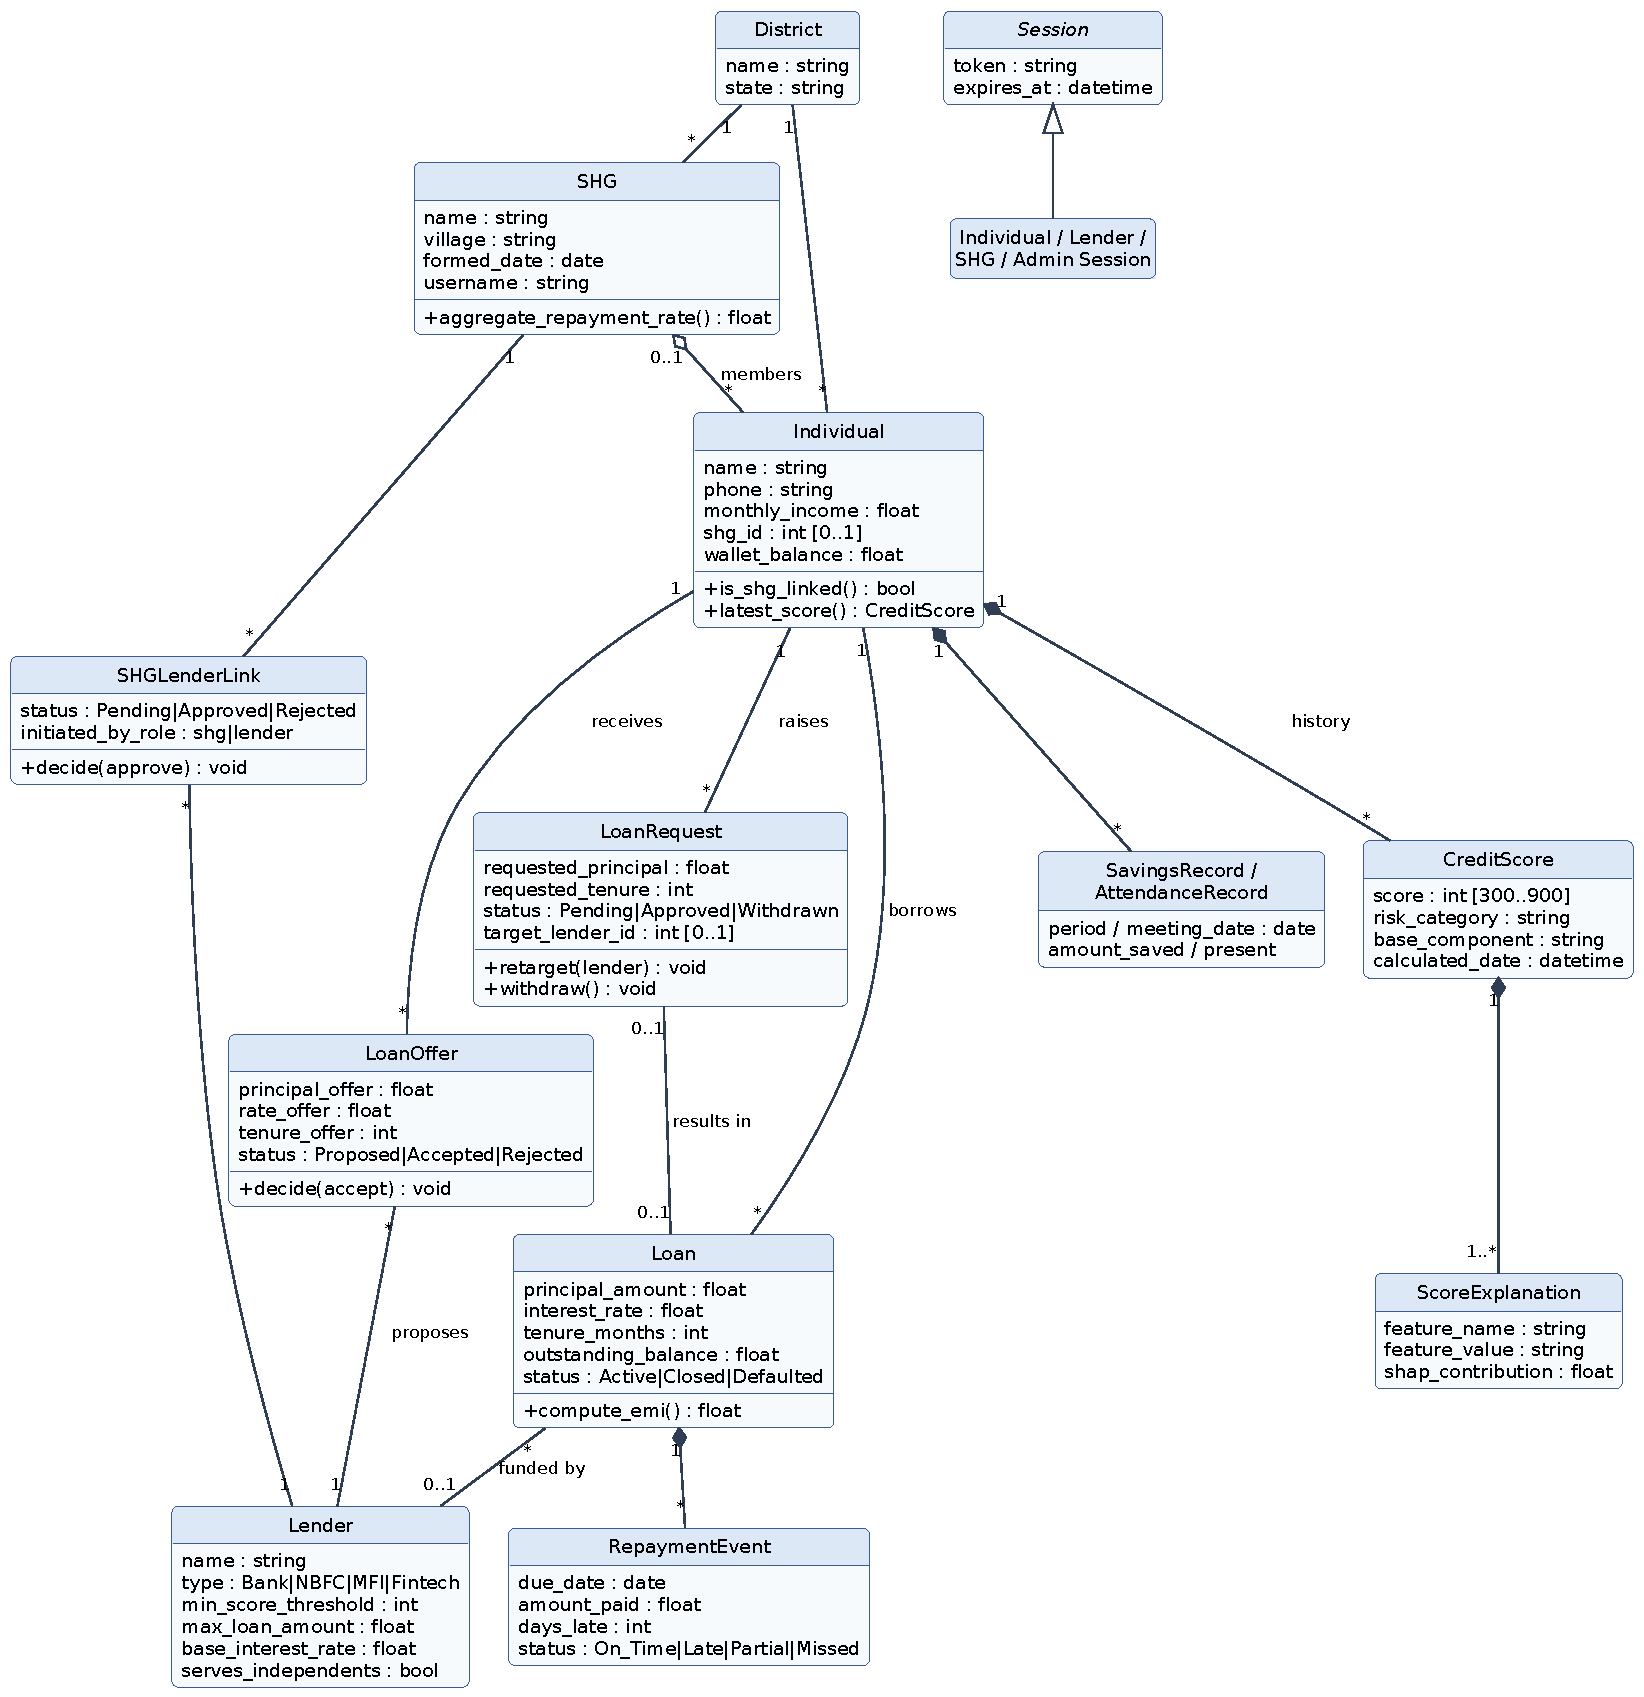
\includegraphics[width=\textwidth]{fig/class_c.pdf}
\caption{Class diagram (domain model)}
\label{fig:class}
\end{figure}

\clearpage
\section{Activity Diagram}
\label{sec:activity-diagram}

Figure~\ref{fig:activity} shows the credit-scoring activity described in
Section~\ref{sec:scoring}: the branch on SHG membership selects the
starting score, and the branch on repayment history decides whether the
model is called at all, which is how the cold-start case is handled without
a separate code path.

\begin{figure}[H]
\centering
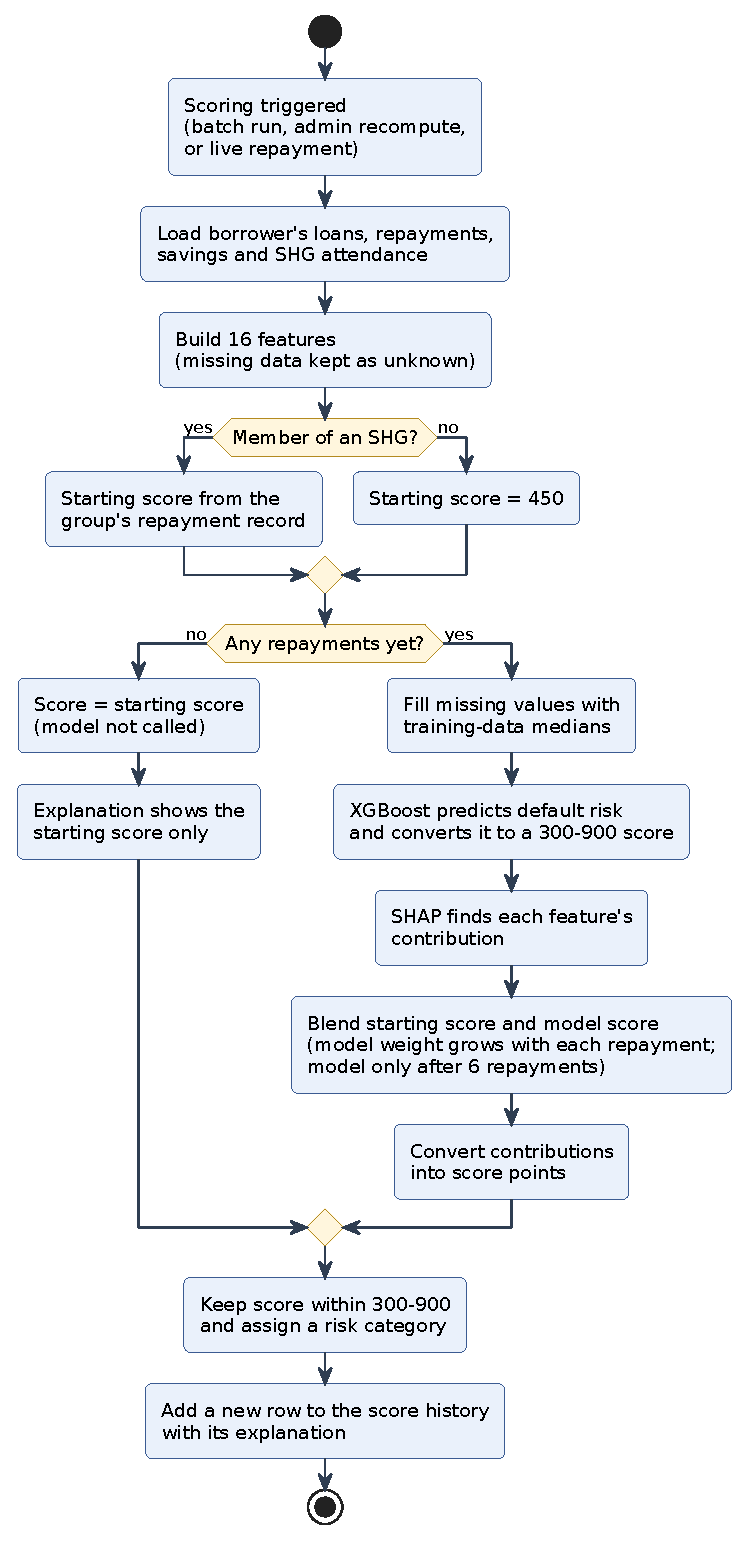
\includegraphics[height=0.78\textheight]{fig/activity_score.pdf}
\caption{Activity diagram: computing a borrower's credit score}
\label{fig:activity}
\end{figure}

\clearpage
Figure~\ref{fig:swimlane} shows the same notation applied to the main
business process, with one swimlane per participant: the borrower's loan
request, the lender's decision, and the repayment that updates the loan,
the wallet and the score in a single transaction. The two stop nodes on the
left of the diagram are the guards described in
Section~\ref{sec:method}: an invalid or ineligible request never reaches a
lender's queue, and a wallet that cannot cover the borrower's total dues
blocks every payment rather than only the one clicked.

\begin{figure}[H]
\centering
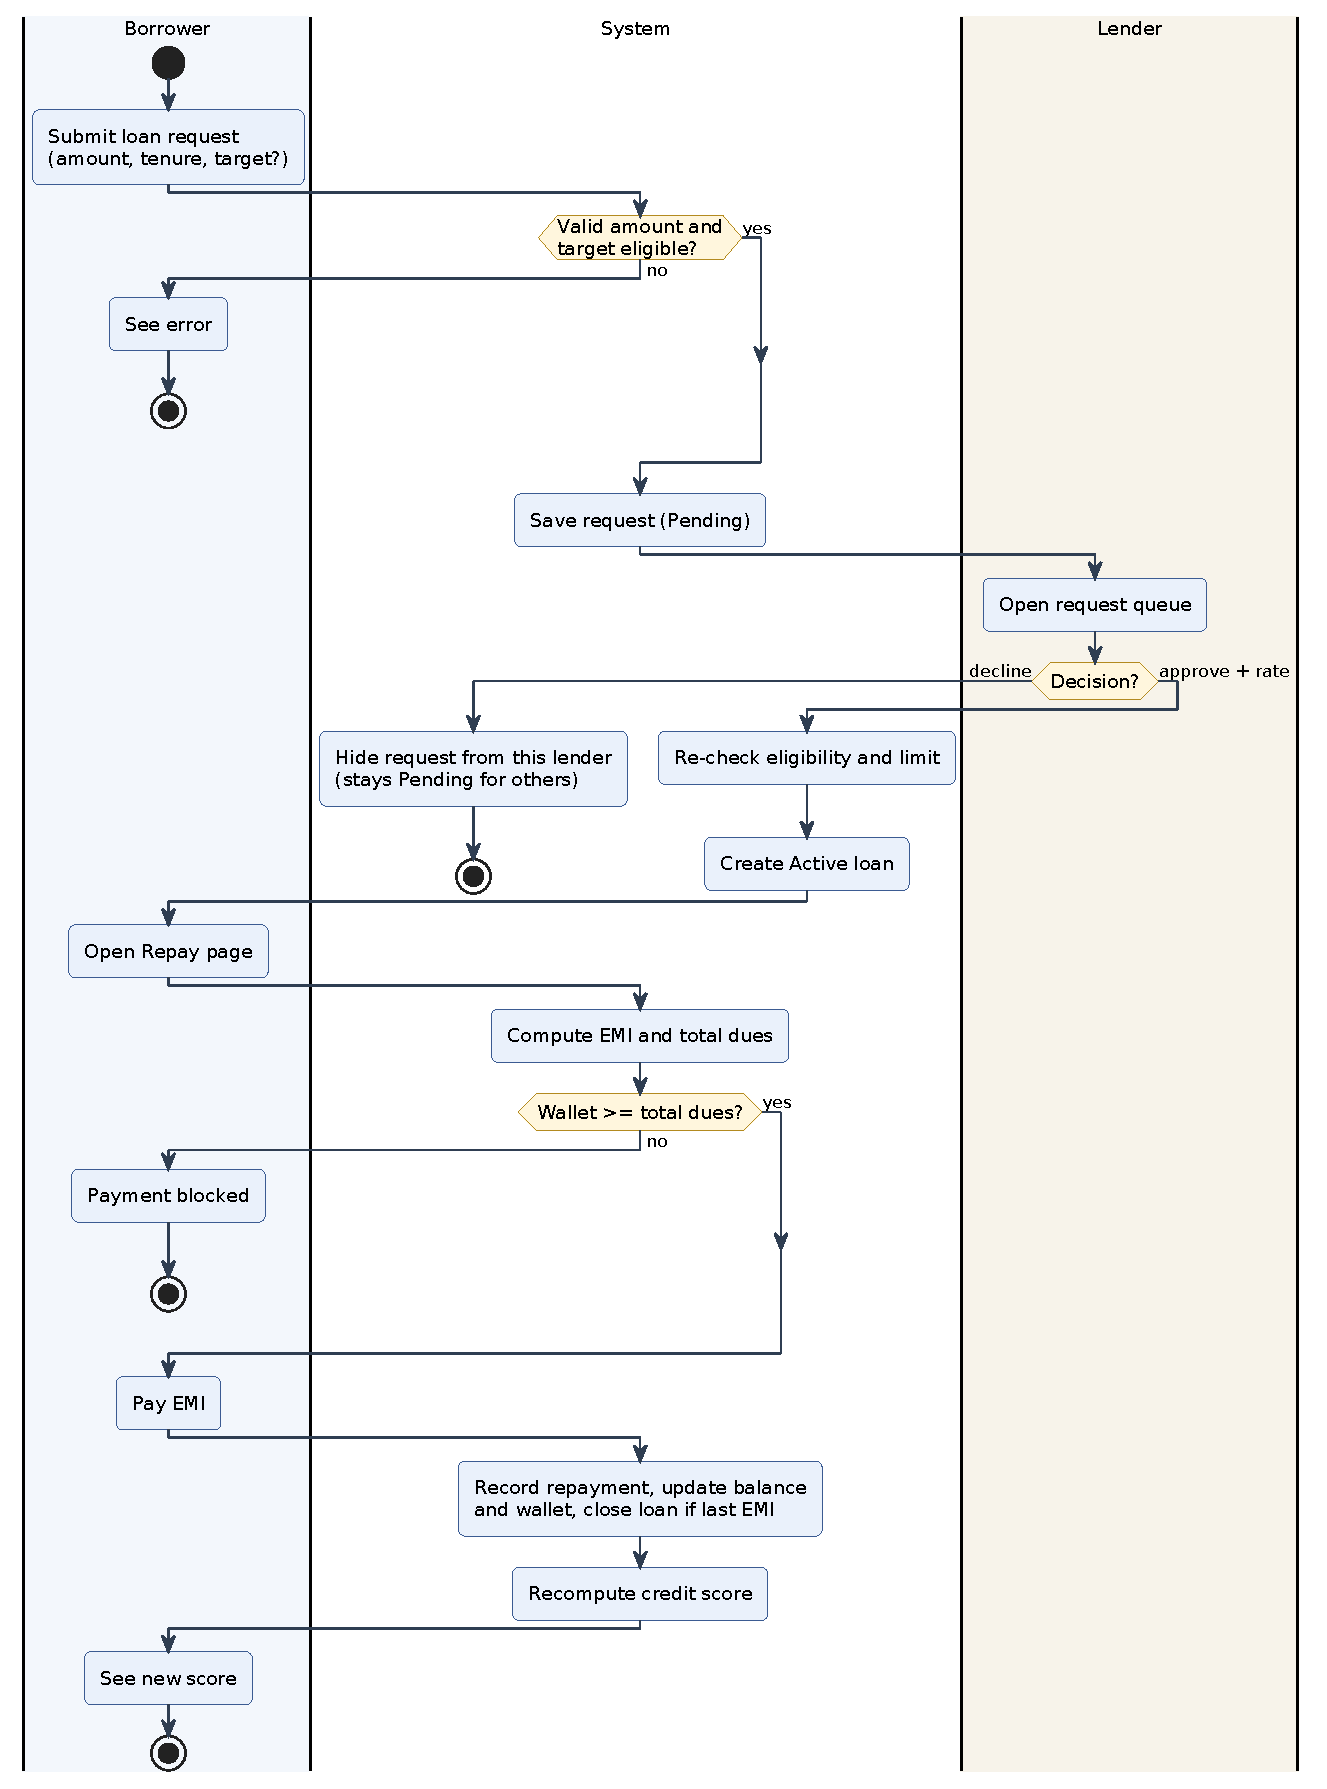
\includegraphics[height=0.80\textheight]{fig/swimlane_c.pdf}
\caption{Activity (swimlane) diagram: loan request, approval and live repayment}
\label{fig:swimlane}
\end{figure}

\clearpage
\addcontentsline{toc}{section}{References}
\begin{thebibliography}{99}
\bibitem{xgboost} Chen, T.; Guestrin, C. XGBoost: A scalable tree boosting system. In \emph{Proceedings of the 22nd ACM SIGKDD International Conference on Knowledge Discovery and Data Mining}, 2016, pp.~785--794.
\bibitem{shap} Lundberg, S.~M.; Lee, S.-I. A unified approach to interpreting model predictions. \emph{Advances in Neural Information Processing Systems} \textbf{2017}, \emph{30}.
\bibitem{treeshap} Lundberg, S.~M.; Erion, G.; Chen, H.; et al. From local explanations to global understanding with explainable AI for trees. \emph{Nature Machine Intelligence} \textbf{2020}, \emph{2}, 56--67.
\bibitem{iforest} Liu, F.~T.; Ting, K.~M.; Zhou, Z.-H. Isolation forest. In \emph{Proceedings of the 8th IEEE International Conference on Data Mining}, 2008, pp.~413--422.
\bibitem{kmeans} Lloyd, S. Least squares quantization in PCM. \emph{IEEE Transactions on Information Theory} \textbf{1982}, \emph{28}, 129--137.
\bibitem{pbkdf2} Moriarty, K.; Kaliski, B.; Rusch, A. PKCS \#5: Password-Based Cryptography Specification Version 2.1. RFC 8018, IETF, 2017.
\bibitem{ieee830} IEEE Recommended Practice for Software Requirements Specifications. IEEE Std 830-1998.
\bibitem{uml} Object Management Group. \emph{Unified Modeling Language (UML) Specification}, Version 2.5.1, 2017.
\bibitem{pressman} Pressman, R.~S.; Maxim, B.~R. \emph{Software Engineering: A Practitioner's Approach}, 9th ed.; McGraw-Hill, 2019.
\bibitem{fastapi} Ram\'{\i}rez, S. FastAPI documentation. \url{https://fastapi.tiangolo.com/}.
\bibitem{sklearn} Pedregosa, F.; et al. Scikit-learn: Machine learning in Python. \emph{Journal of Machine Learning Research} \textbf{2011}, \emph{12}, 2825--2830.
\bibitem{rbi} Reserve Bank of India. Master Directions -- Priority Sector Lending -- Targets and Classification, 2020.
\end{thebibliography}

\end{document}
